\documentclass[12pt, titlepage]{article}

\usepackage[margin=1in]{geometry}
\usepackage[round]{natbib}
\usepackage{multirow}
\usepackage{booktabs}
\usepackage{tabularx}
\usepackage{graphicx}
\usepackage{float}
\usepackage{hyperref}
\usepackage{listings}
\usepackage{amssymb}

\hypersetup{
    colorlinks,
    citecolor=blue,
    filecolor=black,
    linkcolor=red,
    urlcolor=blue
}

%% Comments

\usepackage{color}

\newif\ifcomments\commentstrue %displays comments
%\newif\ifcomments\commentsfalse %so that comments do not display

\ifcomments
\newcommand{\authornote}[3]{\textcolor{#1}{[#3 ---#2]}}
\newcommand{\todo}[1]{\textcolor{red}{[TODO: #1]}}
\else
\newcommand{\authornote}[3]{}
\newcommand{\todo}[1]{}
\fi

\newcommand{\wss}[1]{\authornote{blue}{SS}{#1}} 
\newcommand{\plt}[1]{\authornote{magenta}{TPLT}{#1}} %For explanation of the template
\newcommand{\an}[1]{\authornote{cyan}{Author}{#1}}

%% Common Parts

\newcommand{\progname}{Software Engineering} % PUT YOUR PROGRAM NAME HERE
\newcommand{\authname}{Team 21, Alkalytics
\\ Sumanya Gulati - gulats10
\\ Kate Min - mink9
\\ Jennifer Ye - yej52
\\ Jason Tran - tranj78} % AUTHOR NAMES                  

\usepackage{hyperref}
    \hypersetup{colorlinks=true, linkcolor=blue, citecolor=blue, filecolor=blue,
                urlcolor=blue, unicode=false}
    \urlstyle{same}
                                


\newcounter{acnum}
\newcommand{\actheacnum}{AC\theacnum}
\newcommand{\acref}[1]{AC\ref{#1}}

\newcounter{ucnum}
\newcommand{\uctheucnum}{UC\theucnum}
\newcommand{\uref}[1]{UC\ref{#1}}

\newcounter{mnum}
\newcommand{\mthemnum}{M\themnum}
\newcommand{\mref}[1]{M\ref{#1}}

\begin{document}

\title{Module Guide for \progname{}} 
\author{\authname}
\date{\today}

\maketitle

\pagenumbering{roman}

\section{Revision History}

\begin{tabularx}{\textwidth}{p{3cm}p{2cm}X}
\toprule {\bf Date} & {\bf Version} & {\bf Notes}\\
\midrule
11 January 2025 & 1.0 & Added initial content for Rev 0.\\
17 January 2025 & 1.1 & Finalized document for Rev 0 submission.\\
18 January 2025 & 1.2 & Refined the document.\\
1 April 2025 & 1.3 & Updated document to adhere to
\href{https://github.com/SumanyaG/Alkalytics/issues/176}{176},
\href{https://github.com/SumanyaG/Alkalytics/issues/177}{177},
\href{https://github.com/SumanyaG/Alkalytics/issues/252}{252}, and
\href{https://github.com/SumanyaG/Alkalytics/issues/253}{253}. \\
4 April 2025 & 1.4 & Updated document to adhere to 
\href{https://github.com/SumanyaG/Alkalytics/issues/173}{173},
\href{https://github.com/SumanyaG/Alkalytics/issues/174}{174},
\href{https://github.com/SumanyaG/Alkalytics/issues/178}{178},
\href{https://github.com/SumanyaG/Alkalytics/issues/250}{250},
\href{https://github.com/SumanyaG/Alkalytics/issues/251}{251},
\href{https://github.com/SumanyaG/Alkalytics/issues/252}{252},
\href{https://github.com/SumanyaG/Alkalytics/issues/254}{254} and 
\href{https://github.com/SumanyaG/Alkalytics/issues/255}{255}. \\
\bottomrule
\end{tabularx}
\\
\newline \newline
\emph{\textbf{Note:}} Please note that our team has adapted and extended this
Module Guide document to include the contents of an MIS or other such document.
For this reason, only one design document has been submitted.
\newpage

\section{Reference Material}

This section records information for easy reference.

\subsection{Abbreviations and Acronyms}

\renewcommand{\arraystretch}{1.2}
\begin{tabular}{l l} 
  \toprule		
  \textbf{symbol} & \textbf{description}\\
  \midrule 
  AC & Anticipated Change\\
  API & Application Programming Interface\\
  CSV & Comma Separated Values\\
  DAG & Directed Acyclic Graph \\
  FR & Functional Requirement\\
  JSON & JavaScript Object Notation\\
  KPI & Key Performance Indicator\\
  M & Module \\
  MG & Module Guide \\
  MIS & Module Interface Specification\\
  OS & Operating System \\
  SC & Scientific Computing \\
  SRS & Software Requirements Specification\\
  \progname & Explanation of program name\\
  UC & Unlikely Change \\
  UI & User Interface\\
  XML & Extensible Markup Language\\
  \bottomrule
\end{tabular}\\

\newpage

\tableofcontents

\listoftables

\listoffigures

\newpage

\pagenumbering{arabic}

\section{Introduction}

\subsection{Summary}
Alkalytics is a project designed to provide a scalable data management and analysis
solution for ocean alkalinity research, in particular by streamlining the data 
organization, querying, and visualization processes. Through its various modules, 
the primary goal of the system is to offer a comprehensive solution for data 
ingestion, processing and reporting  while maintaining adaptability to future 
changes.\\
\newline
Each functional component is developed as an independent module to encapsulate 
specific responsibilities, minimize dependencies, and promote information
hiding. This modular approach, advocated for widely in the software sector, not only
simplifies development and testing but also allows the system to accommodate evolving
user requirements and technology upgrades.\\
\newline
A work context model and a use case diagram for the system have been included in the 
\href{https://github.com/SumanyaG/Alkalytics/blob/main/docs/SRS/SRS.pdf}{Software Requirements Specification (SRS)} 
in sections 6.2 and 8.1, respectively.

\subsection{Purpose}
This Module Guide (MG) has been written to serve as a roadmap for the Alkalytics system,
detailing its structure, functionality, and the relationships between its components.
It provides clarity on how the system meets the requirements outlined in the SRS
and supports the following stakeholders:
\begin{itemize}
  \item \textbf{New Developers}: To understand the modular architecture and ensure
  consistent implementation.
  \item \textbf{Maintainers}: To efficiently identify, update, or rewrite modules as needed.
  \item \textbf{Designers}: To validate the system's feasibility, flexibility, and alignment
  with project goals. 
\end{itemize}

\section{Anticipated and Unlikely Changes} \label{SecChange}

This section identifies potential changes to the system and classifies them into
two categories: anticipated changes (AC) as listed in section \ref{SecAchange} and
unlikely changes (UC) as listed in section \ref{SecUchange}. AC represent decisions 
that have been encapsulated within specific modules to minimize the impact of 
modifications while UC are those that, while possible, are fixed at the system 
architecture stage to reduce complexity.

\subsection{Anticipated Changes} \label{SecAchange}

Anticipated changes are the source of the information that is to be hidden
inside the modules. Ideally, changing one of the anticipated changes will only
require changing the one module that hides the associated decision. These changes
are encapsulated within specific modules to ensure the system's adaptability.

\begin{description}
  \item[\refstepcounter{acnum} \actheacnum \label{acHardware}:] \textbf{Hardware Configuration} - 
  The software may need to run on a different hardware platform like a server or on a 
  cloud solution. Changes in hardware specifications will primarily affect the System Interface 
  Module, isolating their imoact.
  
  \item[\refstepcounter{acnum} \actheacnum \label{acProcessing}:] \textbf{Data Processing Algorithms} - 
  Changes in analytical techniques along with advances in the machine learning space would
  introduce the need for new statistical models. These changes would be encapsulated in the
  Data Processing Module.

  \item[\refstepcounter{acnum} \actheacnum \label{acInterface}:] \textbf{User Interface (UI) Design} - 
  Changes in analytical techniques along with advances in the machine learning space would
  introduce the need for new statistical models. These changes would be encapsulated in the
  Data Processing Module.

  \item[\refstepcounter{acnum} \actheacnum \label{acInput}:] \textbf{Input Data Formats} - 
  Currently, the system is expected to process data from Comma Separated Values (CSV) files only.
  In the future, however, modifications may have to be made to accommodate different file 
  formats (such as JavaScript Object Notation (JSON), Extensible Markup Language (XML) etc)
  which will be handled by the Data Ingestion Module without impacting other parts of the system.

  \item[\refstepcounter{acnum} \actheacnum \label{acScaling}:] \textbf{Scaling Data Volume} - 
  As the number of experiments increases, the system may need to handle increasing data volumes
  as usage grows. This is addressed by the Data Storage Module which has been designed to support
  database scalability strategies.

  \item[\refstepcounter{acnum} \actheacnum \label{acRoles}:] \textbf{User Roles and Permissions} - 
  Future requirements may demand the addition of new user roles or changes to existing permissions.
  The Administration Module is designed to encapsulate these changes.

  \item[\refstepcounter{acnum} \actheacnum \label{acSchema}:] \textbf{Input Schema} - 
  With an increase in the number of diverse experiments, the schema for the data inputs may have to
  changed to support the addition or removal of new parameters. This is handled by the Data Ingestion
  Module.

  \item[\refstepcounter{acnum} \actheacnum \label{acNotifs}:] \textbf{Notification Rules} - 
  The conditions of triggering alerts or notifications may evolve, including but not limited to
  additional thresholds or new types of anomalies. These are handled by the Notifications Module
  without affecting other parts of the system.
  
  \item[\refstepcounter{acnum} \actheacnum \label{acMetrics}:] \textbf{Analytical Metrics} - 
  New metrics or Key Performance Indicators (KPIs) might be requested by stakeholders. This would
  involve adapting requirements by introducing new calculations or processing pipelines by modifying
  the Data Processing Module.
  
\end{description}

\subsection{Unlikely Changes} \label{SecUchange}

Unlikely changes are those that are fixed early in the design to simplify the system
and reduce complexity. These changes, if necessary, would have a significant impact on
multiple modules.

\begin{description}
  \item[\refstepcounter{ucnum} \uctheucnum \label{ucIO}:] \textbf{Input/Output Devices} - 
  The system is designed to support file-based inputs. Changes can include additional input
  and/or output methods such as direct hardware interaction, would require substantial
  redesign across multiple modules.
  
  \item[\refstepcounter{ucnum} \uctheucnum \label{ucSysArch}:] \textbf{Core System Architecture} -
  The underlying architectural decisions, such as the use of modular decomposition and separation
  of concerns, are not expected to change. Altering these decisions would necessitate a complete overhaul
  of the system.
  
  \item[\refstepcounter{ucnum} \uctheucnum \label{ucComms}:] \textbf{Communication Protocols} -
  The communication methods between modules such as function calls, API interactions etc are fixed. 
  Switching to a different communication protocol would impact the interfaces of all interacting modules.

  \item[\refstepcounter{ucnum} \uctheucnum \label{ucLanguage}:] \textbf{Programming Language} -
  The choice of programming languages is asssumed to be fixed for the project. A change would
  require rewriting most of the system.

  \item[\refstepcounter{ucnum} \uctheucnum \label{ucDatabase}:] \textbf{Database Type} -
  The choice of storage solution (relational versus NoSQL databases, for example) is assumed to remain
  fixed. Switching to a different type of database would require reworking the Data Storage
  Module and parts of the Data Processing Module.

\end{description}

\section{Module Hierarchy} \label{SecMH}

This section provides an overview of the module design for the Alkalytics system.
The modules are summarized in a hierarchy that follows the principle of information
hiding. Each module encapsulates specific secrets, ensuring changes are localized
and do not affect unrelated parts of the system. These modules are summarized in
a hierarchy decomposed by secrets in table \ref{TblMH}. This hierarchy represented
as a directed acyclic graph, shown in \ref{fig:FigMH}, shows relationships betweem
higher-level and lower-level modules, with the leaf modules representing those that
will actually be implemented.

\begin{description}
\item [\refstepcounter{mnum} \mthemnum \label{mHH}:] System Interface Module
\item [\refstepcounter{mnum} \mthemnum \label{mBH}:] Logic Encapsulation Module
\item [\refstepcounter{mnum} \mthemnum \label{mIN}:] Interface Module 
\item [\refstepcounter{mnum} \mthemnum \label{mAD}:] Administration Module 
\item [\refstepcounter{mnum} \mthemnum \label{mDA}:] Data Acquisition Module 
\item [\refstepcounter{mnum} \mthemnum \label{mDS}:] Data Storage Module 
\item [\refstepcounter{mnum} \mthemnum \label{mDR}:] Data Retrieval Module 
\item [\refstepcounter{mnum} \mthemnum \label{mINP}:] Input Module 
\item [\refstepcounter{mnum} \mthemnum \label{mPR}:] Processing Module 
\item [\refstepcounter{mnum} \mthemnum \label{mOU}:] Output Module 
\item [\refstepcounter{mnum} \mthemnum \label{mUID}:] UI Design Module
\item [\refstepcounter{mnum} \mthemnum \label{mVI}:] Visualization Module
\item [\refstepcounter{mnum} \mthemnum \label{mUM}:] User Management Module 
\item [\refstepcounter{mnum} \mthemnum \label{mCM}:] Configuration Management Module
\item [\refstepcounter{mnum} \mthemnum \label{mDI}:] Data Ingestion Module
\item [\refstepcounter{mnum} \mthemnum \label{mDV}:] Data Validation Module 
\item [\refstepcounter{mnum} \mthemnum \label{mDT}:] Data Transformation Module 
\item [\refstepcounter{mnum} \mthemnum \label{mML}:] Machine Learning Module
\item [\refstepcounter{mnum} \mthemnum \label{mRE}:] Reporting Module 
\item [\refstepcounter{mnum} \mthemnum \label{mNO}:] Notification Module
\end{description}

\begin{table}[h!]
\centering
\begin{tabular}{p{0.3\textwidth} p{0.3\textwidth} p{0.35\textwidth}}
\toprule
\textbf{Level 1} & \textbf{Level 2} & \textbf{Level 3}\\
\midrule

{System Interface Module} & ~ & ~ \\
& Data Acquisition Module & \\
& Data Storage Module & \\
& Data Retrieval Module & \\
\midrule

{Logic Encapsulation Module} & Input Module & Data Ingestion Module\\
& & Data Validation Module\\
& Processing Module & Data Transformation Module\\
& & Machine Learning Module\\
& Output Module & Reporting Module\\
& & Notifications Module\\
\midrule

{Interface Module} & UI Design Module & \\
& Visualization Module & \\
\midrule

{Administration Module} & User Management Module & \\
& Configuration Management Module & \\
\bottomrule

\end{tabular}
\caption{Module Hierarchy}
\label{TblMH}
\end{table}

\begin{figure}[htbp]
  \centering
  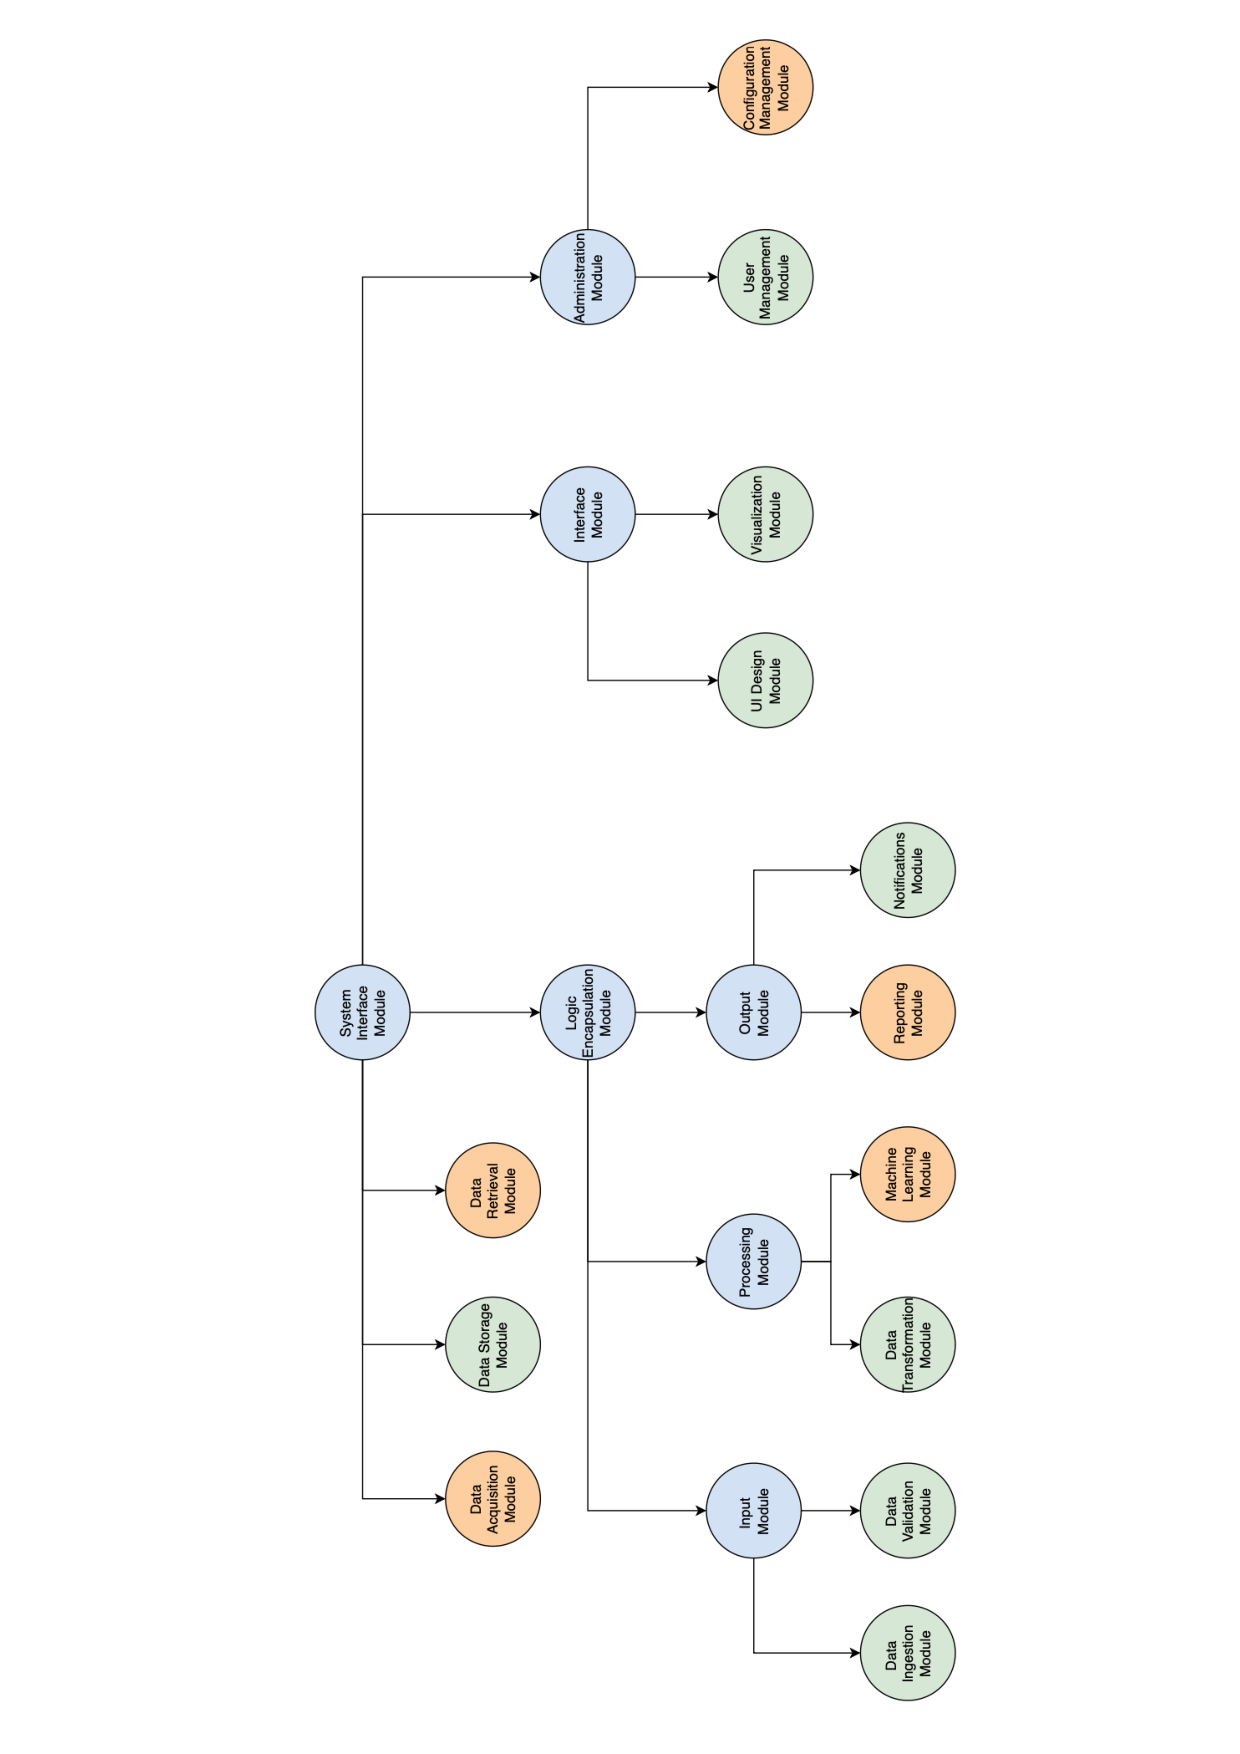
\includegraphics[scale=0.5,angle=-90]{Diagrams/DAG.pdf}
  \caption{A DAG representing the implemented module hierarchy of Alkalytics.}
  \label{fig:FigMH}
\end{figure}

It must be noted that the blue nodes shown in figure \ref{fig:FigMH} represent 
`container' modules that are non-leaf modules and encompass other leaf nodes.
The orange nodes represent leaf modules that will not be implemented for Revision
0 of Alkalytics and the green nodes represent leaf modules that will be implemented.

\section{Module Decomposition} \label{SecMD}

Modules are decomposed according to the principle of ``information hiding''
proposed by \citet{ParnasEtAl1984}. In this section, the \emph{Secrets} field acts as a brief
statement of the design decision hidden by the module. The \emph{Services} field specifies
\emph{what} the module will do without documenting \emph{how} to do it.\\
\newline
For each module, a suggestion for the implementing software is given under the 
\emph{Implemented By} title. If the entry is \emph{OS}, this means that the module is
provided by the operating system or by standard programming language libraries.
\emph{\progname{}} means the module will contain custom code and thus, will be implemented
by the software engineering team.\\
\newline
Descriptions for non-leaf modules or the modules that will not be implemented for Revision 0 of
Alkalytics have been provided below.

\subsection{Data Storage Module (\mref{mDS})}
\begin{description}
  \item[Secrets:] The data structure and algorithm used to store the received CSV files into the
  NoSQL database.
  \item[Services:] This module handles the storage of system data by interacting with
  a NoSQL database. It receives the transformed data from the Data Ingestion Module in a suitable
  format for storage in the database. This module also provides interfaces to query, retrieve, and
  update stored data.
  \item[Implemented By:] Software Engineering
  \item[Rationale:] This module abstracts the complexities of the NoSQL database
  structure, ensuring flexibility in storage design. It allows the system to 
  efficiently store the data in a schema-less NoSQL database. This ensures scalability and 
  adaptability to handle large datasets with varying structures.
\end{description}

\subsubsection{Uses}
This module is used by the Logic Encapsulation and Interface Module to interact
with the stored data. It provides mechanisms transform the CSV data, and
perform CRUD (Create, Read, Update, Delete) operations on the NoSQL database.

\subsubsection{Syntax}
\begin{description}
  \item[Exported Constants and Access Programs:]
  \item 
  \texttt{DB\_CONNECTION\_STRING}: The connection string for accessing the
    NoSQL database.
  \item
  \texttt{MAX\_BATCH\_SIZE}: The maximum number of rows to process and upload
  in a single batch.

  \begin{table}[h!]
    \centering
    \begin{tabular}{p{0.175\textwidth} p{0.175\textwidth} p{0.175\textwidth} p{0.375\textwidth}}
    \toprule
    \textbf{Name} & \textbf{In} & \textbf{Out} & \textbf{Exceptions}\\
    \midrule
    
    \texttt{initializeDB} & - & Boolean & \texttt{DatabaseInitializationError} \\
    \midrule
    
    \texttt{uploadData} & filePath(string) & Boolean &
    \texttt{FileNotFoundError} or \texttt{DataTransformationError} \\
    \midrule

    \texttt{queryData} & query(string) & Data (JSON) & \texttt{QueryExecutionError}\\
    \midrule

    \texttt{updateData} & query(string), updates & Boolean & \texttt{UpdateError} \\
    \bottomrule
    
    \end{tabular}
    \caption{Exported Access Programs for the Data Storage Module}
    \label{TblEAP_Storage}
  \end{table}
\end{description}

\subsubsection{Semantics}
\begin{description}
  \item[State Variables:]
  \item
  \texttt{database}: Represents the connection to the NoSQL database.
  \item
  \texttt{transformationRules}: Defines the set of rules for transforming CSV data to
  JSON format.
  
  \item[Environment Variables:] N/A

  \item[Assumptions:]
  \item
  \begin{itemize}
    \item Assumes the NoSQL database is accessible and the credentials are correct.
  \end{itemize}
  \item
  \begin{itemize}
    \item Assumes the received CSV files are well-formed and follow the expected schema.
  \end{itemize}
  \item 
  \begin{itemize}
    \item Assumes sufficient storage space is available in the database.
  \end{itemize}
  \item 

  \item[Access Routine Semantics:] 
  \item
  \texttt{initializeDB()}:
  \item
  \begin{itemize}
    \item \textbf{Transition}: Establishes a connection to the NoSQL database and validates
    the connection.
  \end{itemize}
  \item
  \begin{itemize}
    \item \textbf{Output}: Returns \texttt{True} if the database is successfully initialized.
  \end{itemize}
  \item
  \begin{itemize}
    \item \textbf{Exception}: Throws a \texttt{DatabaseInitializationError} otherwise.
  \end{itemize}
  \item 

  \texttt{uploadData(filePath:string)}:
  \item
  \begin{itemize}
    \item \textbf{Transition}: Reads the specified CSV file, transforms the contents into
    JSON format using \texttt{transformationRules}, and uploads the transformed data to
    the database in batches.
  \end{itemize}
  \item
  \begin{itemize}
    \item \textbf{Output}: Returns \texttt{True} if successful.
  \end{itemize}
  \item
  \begin{itemize}
    \item \textbf{Exception}: Throws \texttt{FileNotFoundError} if the file does not exist or
    \\ \texttt{DataTransformationError} if the transformation fails.
  \end{itemize}
  \item


\texttt{queryData(query:string)}:
  \item
  \begin{itemize}
    \item \textbf{Transition}: Executes the specified query on the database and retrieves the
    corresponding data.
  \end{itemize}
  \item 
  \begin{itemize}
    \item \textbf{Output}: Returns the retrieved data in JSON format.
  \end{itemize}
  \item
  \begin{itemize}
    \item \textbf{Exception}: Throws \texttt{QueryExecutionError} if the query
    is invalid or fails.
  \end{itemize}
  \item

\texttt{updateData(query:string, updates)}:
  \item
  \begin{itemize}
    \item \textbf{Transition}: Applies the specified updates to the records matching the query
    in the database.
  \end{itemize}
  \item
  \begin{itemize}
    \item \textbf{Output}: Returns \texttt{True} if successful.
  \end{itemize}
  \item
  \begin{itemize}
    \item \textbf{Exception}: Throws \texttt{UpdateError} if the operation fails.
  \end{itemize}
  \item

  \item[Local Function:] 
  \item
\texttt{transformCSVToJSON(filePath:string)}:
  \item
  \begin{itemize}
    \item \textbf{Description}: Reads a CSV file and converts its rows into JSON objects based on
    \texttt{transformationRules}.
  \end{itemize}
  \item 
  \begin{itemize}
    \item \textbf{Output}: Returns a list of JSON objects.
  \end{itemize}
  \item
  \begin{itemize}
    \item \textbf{Exception}: Throws \texttt{DataTransformationError} if the
    transformation fails.
  \end{itemize}
  \item 
  \texttt{validateConnection()}:
  \item 
  \begin{itemize}
    \item \textbf{Description}: Checks the connection to the NoSQL database and returns \texttt{True}
    if valid.
  \end{itemize}
\end{description}

\subsection{Data Ingestion Module (\mref{mDI})} \label{mIngestion}
\begin{description}
  \item[Secrets:] The data structure and algorithm used to ingest and preprocess data from
  the external source (CSV files) into the system.
  \item[Services:] This module is responsible for ingesting external data into the system.
  It interacts with various external data sources and converts incoming data into a 
  standardized format for further processing. The module ensures and facilitates seamless
  data flow into the system for subsequent operations.
  \item[Implemented By:] Software Engineering
  \item[Rationale:] The Data Ingestion Module abstracts the complexities of interacting with
  an external data source enabling the system to ingest data in CSV. By ensuring data Validation
  and transformation, the module guarantees data integrity and consistency before it is processed
  further. It ensures scalability, adaptability and flexibility in handling data from a different
  source while maintaining the quality of ingested data.
\end{description}

\subsubsection{Uses}
The Data Ingestion Module is used by the Data Processing Module to feed raw data into the system
for analysis and storage. It also supports integration with external services to retrieve and
preprocess data as needed. This module, in addition to the Data Validation Module ensures that all
incoming data is correctly formatted and validated before entering the system.

\subsubsection{Syntax}
\textbf{Exported Constants and Access Programs}:
  \begin{table}[H]
    \centering
    \begin{tabular}{p{0.25\textwidth} p{0.21\textwidth} p{0.1\textwidth} p{0.3\textwidth}}
    \toprule
    \textbf{Name} & \textbf{In} & \textbf{Out} & \textbf{Exceptions}\\
    \midrule
    
    \texttt{initializeIngestion} & - & Boolean & \texttt{IngestionError} \\
    \midrule
    
    \texttt{ingestData} & sourcePath(string) & Boolean &
    \texttt{FileNotFoundError} or \texttt{DataTransformationError} \\
    \midrule

    \texttt{validateData} & data(Object) & Boolean &
    \texttt{DataValidationError} \\
    \midrule

    \texttt{retrieveAPIData} & apiEndPoint(string) & Data (JSON) &
    \texttt{APIRequestError} \\
    \midrule

    \texttt{processData} & rawData(Object) & Object &
    \texttt{DataProcessingError} \\
    \bottomrule
    
    \end{tabular}
    \caption{Exported Access Programs for the Data Ingestion Module}
    \label{TblEAP_Ingestion}
\end{table}

\subsubsection{Semantics}
\begin{description}
  \item[State Variables:]
  \item
  \texttt{ingestionSource}: Represents the path or endpoint from which data is ingested.
  \item
  \texttt{dataFormat}: Defines the expected format of incoming data (CSV, in this case).

  \item[Environment Variables:] N/A

  \item[Assumptions:]
  \item
  \begin{itemize}
    \item Assumes the external data sources are available and accessible.
  \end{itemize}
  \item
  \begin{itemize}
    \item Assumes the incoming data follows the expected format and schema.
  \end{itemize}
  \item 
  \begin{itemize}
    \item Assumes adequate network connectivity for external API requests.
  \end{itemize}
  \item
  \begin{itemize}
    \item Assumes sufficient memory and storage to handle large volumes of incoming data.
  \end{itemize}

  \item[Access Routine Semantics:] 
  \item
  \texttt{initializeIngestion()}:
  \item
  \begin{itemize}
    \item \textbf{Transition}: Initialized the data ingestion process by configuring connections to
    external data sources.
  \end{itemize}
  \item
  \begin{itemize}
    \item \textbf{Output}: Returns \texttt{True} if initialization is successful.
  \end{itemize}
  \item
  \begin{itemize}
    \item \textbf{Exception}: Throws an \texttt{IngestionInitializationError} if
    initialization fails.
  \end{itemize}
  \item 

  \texttt{ingestData(sourcePath:string)}:
  \item
  \begin{itemize}
    \item \textbf{Transition}: Reads the specified data source, retrieves the raw data and prepares
    it for processing.
  \end{itemize}
  \item
  \begin{itemize}
    \item \textbf{Output}: Returns \texttt{True} if successful.
  \end{itemize}
  \item
  \begin{itemize}
    \item \textbf{Exception}: Throws \texttt{FileNotFoundError} if the source
    path is invalid or does not exist, or \texttt{DataTransformationError} if
    the transformation process fails.
  \end{itemize}
  \item

  \texttt{retrieveAPIData(apiEndPoint:string)}:
  \item
  \begin{itemize}
    \item \textbf{Transition}: Sends a request to the specified API endpoints and retrieves data in JSON
    format.
  \end{itemize}
  \item 
  \begin{itemize}
    \item \textbf{Output}: Returns the retrieved data in JSON format.
  \end{itemize}
  \item
  \begin{itemize}
    \item \textbf{Exception}: Throws \texttt{APIRequestError} if the request fails.
  \end{itemize}
  \item

  \texttt{processData(rawData:Object)}:
  \item
  \begin{itemize}
    \item \textbf{Transition}: Processes the raw data by applying transformation rules such as data
    normalization, mapping, filtering and more.
  \end{itemize}
  \item
  \begin{itemize}
    \item \textbf{Output}: Returns the processed data in the appropriate format.
  \end{itemize}
  \item
  \begin{itemize}
    \item \textbf{Exception}: Throws \texttt{DataProcessingError} if the processing fails.
  \end{itemize}
  \item

  \item[Local Function:] 
  \item
  \texttt{transformRawDataToStandardFormat(sourcePath:string)}:
  \item
  \begin{itemize}
    \item \textbf{Description}: Reads the raw data from the specified source and applies the necessary Transformation
    rules and converts the data into a standardized format.
  \end{itemize}
  \item 
  \begin{itemize}
    \item \textbf{Output}: Returns the transformed data as a JSON object.
  \end{itemize}
  \item
  \begin{itemize}
    \item \textbf{Exception}: Throws \texttt{DataTransformationError} if the
    transformation fails.
  \end{itemize}
  \item 

  \texttt{validateSourceConnection()}:
  \item 
  \begin{itemize}
    \item \textbf{Description}: Checks the connection to the external data source and returns \texttt{True} if valid.
  \end{itemize}
  \item 
  \begin{itemize}
    \item \textbf{Output}: Returns \texttt{True} if the connection to the source is valid.
  \end{itemize}
  \item
  \begin{itemize}
    \item \textbf{Exception}: Throws \texttt{SourceConnectionError} if the
    connection fails.
  \end{itemize}
\end{description}

\subsection{Data Validation Module (\mref{mDV})}
\begin{description}
  \item[Secrets:] The data structure is a finite-state machine designed to model transitions based on real-time 
  input data. The algorithm uses discrete math principles to validate parameters by comparing them against predefined
  thresholds and conditions derived from system requirements.
  \item[Services:] This module ensures valid data is provided for processing by validating input streams, flagging
  anomalies, and initiating corrective actions when necessary.
  \item[Implemented By:] OS and Software Engineering
  \item[Rationale:] Ensuring the integrity and realiability of input data is critical for accurate system operation.
  The FSM representation enables systematic handling of transitions, facilitating robust validation and error 
  detection mechanisms.
\end{description}

\subsubsection{Uses}
It is used to validate the sensor readings against operational thresholds while monitoring real-time 
data streams for deviations or inconsistencies. This module serves as a pre-processing step to ensure 
clean input data  for dependent modules.

\subsubsection{Syntax}
\begin{description}
  \item[Exported Constants and Access Programs:]
  \item 
  \texttt{MAX\_VOLTAGE}: Maximum allowable voltage (e.g., 10 V).
  \item
  \texttt{MIN\_VOLTAGE}: Minimum allowable voltage (e.g., 0 V).
  \item
  \texttt{MAX\_CURRENT}: Maximum allowable current (e.g., 1 A).
  \item
  \texttt{MIN\_CURRENT}: Minimum allowable current (e.g., 0 A).
  \item
  \texttt{MAX\_FLOW\_RATE\_THRESHOLD}: Maximum flow rate (e.g., 0.1 L/min).
  \item
  \texttt{MIN\_FLOW\_RATE\_THRESHOLD}: Minimum flow rate (e.g., 60 L/min).
  \item
  \texttt{MIN\_PH}: Minimum pH range (e.g., 6.0).
  \item
  \texttt{MAX\_PH}: Maximum pH range (e.g., 8.5).

  \begin{table}[H]
    \centering
    \begin{tabular}{p{0.2\textwidth} p{0.2\textwidth} p{0.175\textwidth} p{0.3\textwidth}}
    \toprule
    \textbf{Name} & \textbf{In} & \textbf{Out} & \textbf{Exceptions}\\
    \midrule
    
    \texttt{validateVoltage} & v($\mathbb{R}$) & Boolean & - \\
    \midrule
    
    \texttt{validateCurrent} & i($\mathbb{R}$) & Boolean & - \\
    \midrule

    \texttt{validateFlowRate} & f($\mathbb{R}$) & Data (JSON) & - \\
    \midrule

    \texttt{validatePH} & ph($\mathbb{R}$) & Boolean & - \\

    \midrule
    
    \texttt{getErrorFlags} & - & Set & - \\
    \bottomrule
    
    \end{tabular}
    \caption{Exported Access Programs for the Data Validation Module}
    \label{TblEAP_Validation}
  \end{table}
\end{description}

\subsubsection{Semantics}
\begin{description}

  \item[State Variables:]
  \item
    \begin{itemize}
      \item \texttt{voltage}: Current voltage reading.
    \end{itemize}
    \item
    \begin{itemize}
      \item \texttt{current}: Current current reading.
    \end{itemize}
    \item 
    \begin{itemize}
      \item \texttt{flow\_rate}: Current flow rate reading.
    \end{itemize}
    \item 
    \begin{itemize}
      \item \texttt{ph}: Current pH value.
    \end{itemize}
    \item 
    \begin{itemize}
      \item \texttt{error\_flags}: Set of flags indicating validation failures.
    \end{itemize}
  
  \item[Environment Variables:] N/A

  \item[Assumptions:]
  \item
    \begin{itemize}
      \item Sensors provide data at consistent intervals.
    \end{itemize}
    \item
    \begin{itemize}
      \item Thresholds are pre-configured and static unless updated manually.
    \end{itemize}
    \item 
    \begin{itemize}
      \item Input data is numeric and within hardware limits.
    \end{itemize}

  \item[Access Routine Semantics:]
  \item
    \begin{itemize}
      \item \texttt{validateVoltage(v: Any)}:
      \begin{itemize}
        \item output := \texttt{isReal(v)} $\land$ \texttt{MIN\_VOLTAGE} $\leq$ \texttt{toReal(v)} $\leq$ \texttt{MAX\_VOLTAGE}
        \item if $\lnot$ \texttt{isReal(v)}: \texttt{error\_flags} $\mathrel{+}= \texttt{Voltage\_Type\_Error}$
        \item else if $\lnot$ (\texttt{MIN\_VOLTAGE} $\leq$ \texttt{toReal(v)} $\leq$ \texttt{MAX\_VOLTAGE}): \texttt{error\_flags} $\mathrel{+}= \texttt{Voltage\_Range\_Error}$
      \end{itemize}
    \end{itemize}

    \item
    
    \begin{itemize}
      \item \texttt{validateCurrent(i: Any)}:
      \begin{itemize}
        \item output := \texttt{isReal(i)} $\land$ \texttt{MIN\_CURRENT} $\leq$ \texttt{toReal(i)} $\leq$ \texttt{MAX\_CURRENT}
        \item if $\lnot$ \texttt{isReal(i)}: \texttt{error\_flags} $\mathrel{+}= \texttt{Current\_Type\_Error}$
        \item else if $\lnot$ (\texttt{MIN\_CURRENT} $\leq$ \texttt{toReal(i)} $\leq$ \texttt{MAX\_CURRENT}): \texttt{error\_flags} $\mathrel{+}= \texttt{Current\_Range\_Error}$
      \end{itemize}
    \end{itemize}
    
    \item 
    
    \begin{itemize}
    \item \texttt{validateFlowRate(f: Any)}:
      \begin{itemize}
        \item output := \texttt{isReal(f)} $\land$ \texttt{FLOW\_RATE\_THRESHOLD}[0] $\leq$ \texttt{toReal(f)} $\leq$ \texttt{FLOW\_RATE\_THRESHOLD}[1]
        \item if $\lnot$ \texttt{isReal(f)}: \texttt{error\_flags} $\mathrel{+}= \texttt{FlowRate\_Type\_Error}$
        \item else if $\lnot$ (\texttt{FLOW\_RATE\_THRESHOLD}[0] $\leq$ \texttt{toReal(f)} $\leq$ \texttt{FLOW\_RATE\_THRESHOLD}[1]): \texttt{error\_flags} $\mathrel{+}= \texttt{FlowRate\_Range\_Error}$
      \end{itemize}
    \end{itemize}
    
    \item

    \begin{itemize}
      \item \texttt{validatePH(p: Any)}:
      \begin{itemize}
        \item output := \texttt{isReal(p)} $\land$ \texttt{PH\_RANGE}[0] $\leq$ \texttt{toReal(p)} $\leq$ \texttt{PH\_RANGE}[1]
        \item if $\lnot$ \texttt{isReal(p)}: \texttt{error\_flags} $\mathrel{+}= \texttt{PH\_Type\_Error}$
        \item else if $\lnot$ (\texttt{PH\_RANGE}[0] $\leq$ \texttt{toReal(p)} $\leq$ \texttt{PH\_RANGE}[1]): \texttt{error\_flags} $\mathrel{+}= \texttt{PH\_Range\_Error}$
      \end{itemize}
    \end{itemize}
    
    \item 
    
    \begin{itemize}
      \item \texttt{getErrorFlags()}:
        \begin{itemize}
          \item output := \texttt{error\_flags}
        \end{itemize}
    \end{itemize}    

  \item[Local Function:]
  \item
  \texttt{isWithinRange(value: Real, range: Tuple[Real, Real])} $\to$ \texttt{Boolean}:\\
  Checks if a given value lies within a specified range.
\end{description}

\subsection{Data Transformation Module (\mref{mDT})}
\begin{description}
  \item[Secrets:] The module uses a structured format to store input data and processed results, ensuring
  efficient access and manipulation during analysis and transformation. In addition to that, the module implements
  algorithms to process raw data, apply transformations, and perform statistical or mathematical operations,
  ultimately generating graph-ready data for the visualization module.
  \item[Services:] The modules handles data transformation and analysis tasks by interfacing directly with both 
  the input data and the visualization module which requires processed data for display. This module performs 
  calculations such as data normalization, aggregation, or statistical analysis, and ensures that data is presented 
  in a format that can be used by the visualization module for graph rendering.
  \item[Implemented By:] OS
  \item[Rationale:] The module is designed to centralize the data transformation and analysis logic, providing the core 
  functionality needed for the system to process raw inputs and generate graphical outputs. By abstracting these tasks 
  from other system components, this module enables a cleaner and more modular architecture, improving maintainability 
  and reusability.
\end{description}

\subsubsection{Uses}
\begin{description}
  \item \textbf{Data Transformation}: The module processes raw input data, applying necessary transformations to make 
  the data ready for analysis. This could include scaling, filtering, or feature extraction.
  \item \textbf{Graph Data Preparation}: Once transformed, the data is formatted for graphing. This could imvolve calculating 
  aggregates, trends, or applying statistical functions to produce actionable insights.
  \item \textbf{Interface with Visualization Module}: The module feeds processed data into the visualization module, which 
  then generates graphical outputs based on the processed data.
\end{description}

\subsubsection{Syntax}
\begin{description}
  \item[Exported Constants and Access Programs:]
  \item
  \texttt{TRANSFORMATION\_TYPE}: Defines the types of transformations available including normalization and filtering.
  \item 
  \texttt{GRAPH\_TYPES}: Constants indicating types of graphs to be generated.

  \begin{table}[h!]
    \centering
    \begin{tabular}{p{0.3\textwidth} p{0.2\textwidth} p{0.175\textwidth} p{0.2\textwidth}}
    \toprule
    \textbf{Name} & \textbf{In} & \textbf{Out} & \textbf{Exceptions}\\
    \midrule
    
    \texttt{transformData} & inputData & transformedData & - \\
    \midrule
    
    \texttt{generatedGraphData} & transformedData & graphData & - \\
    \midrule

    \texttt{startTransformation} & - & - & - \\
    \midrule

    \texttt{retrieveGraphData} & - & - & - \\
    
    \bottomrule
    
    \end{tabular}
    \caption{Exported Access Programs for the Data Transformation Module}
    \label{TblEAP_Transformation}
  \end{table}
\end{description}

\subsubsection{Semantics}
\begin{description}
  \item[State Variables:]
  \item \texttt{transformedData}: Holds the data after transformation, ready for graphing.
  \item[Environment Variables:] N/A

  \item[Assumptions:]
  \item
  \begin{itemize}
    \item The input data is assumed to be in a compatible format.
  \end{itemize}
  \item 
  \begin{itemize}
    \item The system is capable of handling large datasets for transformation without significant 
    performance degradation.
  \end{itemize}
  \item 

  \item[Access Routine Semantics:] 
  \item \texttt{startTransformation()}: Initiates the data transformation process which must be completed before 
  any graph generation can occur.
  \item \texttt{retrieveGraphData()}: Returns the transformed data that is now ready to be passed to the visualization 
  module.
  \item
  \item[Local Function:] 
  \item \texttt{applyTransformation()}: Applies a specific transformation to the data.
  \item \texttt{prepareGraphData()}: Formats the transformed data into a structure that the visualization module can use.
\end{description}

\subsection{Notifications Module (\mref{mNO})}
\textbf{OUT OF SCOPE}
\begin{description}
  \item[Secrets:] Each notification is associated with metadata such as the type of notification 
  (info, warning, error), the recipient and the message content. This means the module uses 
  event-driven algorithms to trigger notifications based on system actions or states. 
  \item[Services:] This module provides notifications to users based on predefined events or actions 
  within the system. Notifications can include real-time alerts, status updates or reminders and 
  can be filtered or categorized allowing users to specify which types of notifications they 
  wish to receive.
  \item[Implemented By:] Software Engineering. The module may also rely on external libraries or APIs 
  for delivering emails or push notifications. A few examples of such libraries include SendGrid for email 
  or Firebase for push notifications.
  \item[Rationale:] The purpose of this module is to ensure that users are kept up-to-date on critical 
  events, issues and actions within the system. Timely notifications ensure that users can act on 
  important tasks or system status changes without needing to constantly monitor the system.
\end{description}

\subsubsection{Uses}
\begin{itemize}
  \item \textbf{Real-Time Alerts}: To notify users in real time when significant events occur such as 
  when a task is completed or an error is detected.
  \item \textbf{System Status Updates}: To inform users about the current status of ongoing processes. It 
  also ensures that the application complies with Norman's design principles (feedback, to be specific).
  \item \textbf{Error and Issues Notifications}: To alert users about system errors or issues that require 
  immediate attention such as data transformation errors and more.
\end{itemize}

\subsubsection{Syntax}
\begin{description}
  \item[Exported Constants and Access Programs:]
  \item 
  \texttt{NOTIFICATION\_TYPES}: Defines the types of notifications (e.g., "info", "warning", "error", etc.)
  \item \texttt{DELIVERY\_METHODS}: Defines the available notification delivery methods.
  \item \texttt{DEFAULT\_PREFERENCES}: Default notification preferences for users including the 
  frequency of notifications and the types of events they wish to be notified about.

  \begin{table}[H]
    \centering
    \begin{tabular}{p{0.375\textwidth} p{0.2\textwidth} p{0.1\textwidth} p{0.2\textwidth}}
    \toprule
    \textbf{Name} & \textbf{In} & \textbf{Out} & \textbf{Exceptions}\\
    \midrule
    
    \texttt{sendNotification} & type, recipient, message & - & - \\
    \midrule
    
    \texttt{setNotificationPreferences} & user, preference & - & - \\
    \midrule

    \texttt{getPendingNotifications} & user & - & - \\
    \midrule

    \texttt{triggerNotification} & event & - & - \\

    \bottomrule
    
    \end{tabular}
    \caption{Exported Access Programs for the Notifications Module}
    \label{TblEAP_Notifications}
  \end{table}
\end{description}

\subsubsection{Semantics}
\begin{description}
  \item[State Variables:]
  \item \texttt{currentNotifications}: Stores a list of active or pending notifications that need 
  to be sent.
  \item \texttt{userPreferences}: Stores user-specific notification preferences such as preferred 
  delivery method and event types they want to be notified about.
  \item \texttt{notificationQueue}: A queue that holds notifications waiting to be delivered.
  \item[Environment Variables:] N/A
  \item[Assumptions:] 
  \item
  \begin{itemize}
    \item The system assumes that external services like email APIs are available and functional.
  \end{itemize}
  \item 
  \begin{itemize}
    \item It assumes that users are registered in the system and have specified preferences for 
    notifications.
  \end{itemize}
  \item 
  \begin{itemize}
    \item The system will handle retries or failures in sending notifications, ensuring that critical 
    messages are delivered.
  \end{itemize}
  \item 

  \item[Access Routine Semantics:]
  \item \texttt{sendNotification(type, recipient, message)}: This routine sends a notification to a 
  specified recipient with a message. It ensures that the notification is delivered through the correct 
  channel based on the recipient's preferences.
  \item \texttt{setNotificationPreferences(user, preferences)}: This routine updates the user's notification 
  settings, including how they want to receive notifications and which types they wish to receive.
  \item \texttt{getPendingNotifications(user)}: This routine retrieves the list of notifications that are 
  pending delivery for a specific user.
  \item \texttt{triggerNotification(event)}: This routine triggers the sending of a notification based on 
  a system event.
  \item 

  \item[Local Function:] 
  \item \texttt{formatMessage(event)}: Formats the message to be sent in the notification based on the 
  type of event.
  \item \texttt{validatePreferences(preferences)}: Validates the user preferences to ensure that they are 
  correctly set.
\end{description}

\subsection{UI Design Module (\mref{mUID})}
\begin{description}
  \item[Secrets:] The design specifications and UI components that make  up the
  overall appearance and user experience of the system.
  \item[Services:] This module is responsible for the design and layout of the
  user interface.
  \item[Implemented By:] Software Engineering
  \item[Rationale:] The UI Design Module abstracts the presentation of data and
  interactions with the user.
\end{description}

\subsubsection{Uses}
This module is used by the Interface Module to manage the display of data and
user-related actions, ensuring that the design is consistent and offers a
positive user experience.

\subsubsection{Syntax}
\begin{description}
  \item[Exported Constants and Access Programs:]
  \item
  \begin{table}[h!]
    \centering
    \begin{tabular}{p{0.175\textwidth} p{0.175\textwidth} p{0.175\textwidth} p{0.3\textwidth}}
    \toprule
    \textbf{Name} & \textbf{In} & \textbf{Out} & \textbf{Exceptions}\\
    \midrule
    \texttt{renderUI} & [components] & - & \texttt{RenderError} \\
    \midrule
    \texttt{updateUI} & component & - & \texttt{UpdateError} \\
    \bottomrule
    \end{tabular}
    \caption{Exported Access Programs for the UI Design Module}
    \label{TblEAP_UI}
  \end{table}
\end{description}

\subsubsection{Semantics}
\begin{description}
  \item[State Variables:] N/A
  
  \item[Environment Variables:] N/A
  
  \item[Assumptions:]
  \item
  \begin{itemize}
    \item Assumes the frontend framework is correctly set up for rendering UI components.
  \end{itemize}
  
  \item[Access Routine Semantics:] 
  \item \texttt{renderUI()}:
  \begin{itemize}
    \item \textbf{Transition}: Renders the components to display on the user interface.
    \item \textbf{Exception}: Throws \texttt{RenderError} if the UI rendering fails.
  \end{itemize}
  
  \item \texttt{updateUI()}:
  \begin{itemize}
    \item \textbf{Transition}: Updates specific components of the UI based on route changes or user interactions.
    \item \textbf{Exception}: Throws \texttt{UpdateError} if updates fail.
  \end{itemize}
  
  \item[Local Function:] N/A
\end{description}

\subsection{Visualization Module (\mref{mVI})}
\begin{description}
  \item[Secrets:] This module implements data mapping algorithms to convert raw data into visual 
  elements like charts, graphs, and plots. These include scaling, data aggregation, and color-coding 
  based on user preferences or data thresholds.
  \item[Services:] This module provides static and interactive visual representations of data such as 
  charts, graphs, and dashboards enabling users to explore trends, patterns and insights through intuitive 
  visual tools. It also integrates seamlessly with other system modules allowing processed data from 
  the Data Transformation Module to be displayed effectively.
  \item[Implemented By:] Software Engineering. The module also uses inbuilt libraries or frameworks.
  \item[Rationale:] The Visualization Module is essential for conveying complex data insights in an 
  accessible and actionable format. By transforming raw or processed data into visual forms, users can 
  quickly grasp key trends and make informed decisions.
\end{description}

\subsubsection{Uses}
\begin{itemize}
  \item \textbf{Trend Analysis}: To display temporal or spatial trends in datasets.
  \item \textbf{Comparative Analysis}: To compare different datasets or categories using 
  bar charts, pie charts etc.
  \item \textbf{Anomaly Detection}: To highlight outliers or anomalies in datasets through scatter 
  plots or heatmaps.
  \item \textbf{Interactive Dashboards}: To allow users to explore data dynamically using filters, 
  zooming, and drilldowns.
\end{itemize}

\subsubsection{Syntax}
\begin{description}
  \item[Exported Constants and Access Programs:]
  \item \texttt{CHART\_TYPES}: Defines supported chart types.
  \item \texttt{DEFAULT\_STYLES}: Specifies default styles for visualizations including colours, 
  fonts and sizes.
  \item \texttt{INTERACTION\_MODES}: Defines supported user interaction modes
  (e.g., ``hover'', ``zoom'', `'`filter'', etc.).
  \item
  \begin{table}[H]
    \centering
    \begin{tabular}{p{0.3\textwidth} p{0.2\textwidth} p{0.17\textwidth} p{0.2\textwidth}}
    \toprule
    \textbf{Name} & \textbf{In} & \textbf{Out} & \textbf{Exceptions}\\
    \midrule
    \texttt{createChart} & data, chartType, options & chartID & - \\
    \midrule
    \texttt{updateChart} & chartID, newData & - & - \\
    \midrule
    \texttt{addInteraction} & chartID, interactionType & - & - \\
    \midrule
    \texttt{renderDashboard} & dashboardConfig & - & - \\
    \midrule
    \texttt{exportVisualization} & chartID, format & - & - \\
    \bottomrule
    \end{tabular}
    \caption{Exported Access Programs for the Visualization Module}
    \label{TblEAP_Visualization}
  \end{table}
\end{description}

\subsubsection{Semantics}
\begin{description}
  \item[State Variables:]
  \item \texttt{currentVisualizations}: A dictionary that stores all active visualizations along with their 
  metadata.
  \item \texttt{userPreferences}: Stores user-specific preferences for visualization styles, colour schemes,
  and interaction settings.
  \item \texttt{dashboardLayouts}: Maintains the configuration and layout of user-created dashboards.
  \item 

  \item[Environment Variables:] 
  \item \texttt{BROWSER\_SUPPORT}: Ensures compatibility with web browsers for rendering visualizations.
  \item \texttt{GRAPHICS\_LIBRARY}: Specifies the underlying graphics library used for rendering.
  \item \texttt{DATA\_API}: Interface to retrieve data from the Data Transformation Module or other 
  backend services.
  \item 

  \item[Assumptions:]
  \item
  \begin{itemize}
    \item Input data is preprocessed and cleaned by the Data Transformation Module before being passed to the
    Visualization Module.
  \end{itemize}
  \item 
  \begin{itemize}
    \item Users will have access to compatible devices and software capable of rendering visualizations.
  \end{itemize}
  \item 
  \begin{itemize}
    \item The system's graphics library is fully operational and supports the required visualization types.
  \end{itemize}
  \item 

  \item[Access Routine Semantics:] 
  \item \texttt{createChart(data, chartType, options)}:
  \begin{itemize}
    \item \textbf{Inputs}:
    \begin{enumerate}
      \item \texttt{data}: The dataset to be visualized.
      \item \texttt{chartType}: Type of chart to generate.
      \item \texttt{options}: Optional configuration settings such as axis labels, colours etc.
    \end{enumerate}

    \item \textbf{Effects}: Generates a visualization based on the provided inputs and adds it to 
    the \texttt{currentVisualizations}.

    \item \textbf{Outputs}: Returns a unique \texttt{chartID} for the created visualization.
  \end{itemize}

  \item \texttt{updateChart(chartID, newData)}:
  \begin{itemize}
    \item \textbf{Inputs}:
    \begin{enumerate}
      \item \texttt{chartID}: Identifier for the chart to update.
      \item \texttt{newData}: New dataset to render in the chart.
    \end{enumerate}

    \item \textbf{Effects}: Replaces the chart's data with \texttt{newData} and refreshes the 
    visualization.
  \end{itemize}

  \item \texttt{addInteraction(chartID, interactionType)}:
  \begin{itemize}
    \item \textbf{Inputs}:
    \begin{enumerate}
      \item \texttt{chartID}: Identifier for the chart to modify.
      \item \texttt{interactionType}: Type of interaction to enable.
    \end{enumerate}

    \item \textbf{Effects}: Enhances the chart with the specified interaction mode.
  \end{itemize}

  \item \texttt{renderDashboard(dashboardConfig)}:
  \begin{itemize}
    \item \textbf{Inputs}:
    \begin{enumerate}
      \item \texttt{dashboardConfig}: Configuration file defining the layout and contents of 
      the dashboard.
    \end{enumerate}

    \item \textbf{Effects}: Creates a multi-chart dashboard and stores it in \texttt{dashboardLayouts}
  \end{itemize}

  \item \texttt{exportVisualization(chartID, format)}:
  \begin{itemize}
    \item \textbf{Inputs}:
    \begin{enumerate}
      \item \texttt{chartID}: Identifier of the chart to export.
      \item \texttt{format}: Export format.
    \end{enumerate}

    \item \textbf{Effects}: Exports the chart as a file in the specified format.
  \end{itemize}

  \item[Local Function:]
  \item \texttt{scaleData(data, chartType)}: Adjusts the scale and format of input data based on 
  the chart type, e.g., logarithmic scaling for larger ranges.
  \item \texttt{applyStyles(chartID, styles)}: Applies style customizations.
  \item \texttt{validateConfig(dashboardConfig)}: Ensures that the dashboard configuration file is 
  correctly formatted and contains valid references to data and charts.
\end{description}

\subsection{User Management Module (\mref{mUM})}
\begin{description}
  \item[Secrets:] The data structure and algorithm used to store and manage user
  credentials.
  \item[Services:]This module manages the creation, retrieval, and validation of
  user accounts. It interacts with the database to store user information and
  also provides interfaces for user authentication and Role-Based Access
  Control (RBAC).
  \item[Implemented By:] \progname{}
  \item[Rationale:] This module abstracts the management of user data, ensuring
  that sensitive information, such as passwords, is hashed and not stored in
  plain-text. It also enables the management of user access levels within the
  application. 
\end{description}

\subsubsection{Uses}
This module interacts with the System Interface Module for user credential
storage and verification.

\subsubsection{Syntax}
\begin{description}
  \item[Exported Constants and Access Programs:]
  \item 
  \texttt{SESSION\_COOKIE}: The id of the session cookie used to maintain user sessions.
  
  \begin{table}[H]
    \centering
    \begin{tabular}{p{0.175\textwidth} p{0.2\textwidth} p{0.175\textwidth}
    p{0.3\textwidth}}
    \toprule
    \textbf{Name} & \textbf{In} & \textbf{Out} & \textbf{Exceptions}\\
    \midrule
    
    \texttt{createUser} & email(string), password(string), role(string) &
    \texttt{USER} & \texttt{UserAlreadyExistsError} \\
    \midrule
    
    \texttt{validateUser} & email(string), password(string) & Boolean &
    \texttt{UserNotFoundError} or \texttt{IncorrectPasswordError}\\
    \midrule

    \texttt{getUserAndRole} & email(string) & \texttt{USER} &
    \texttt{UserNotFoundError} \\
    \bottomrule

    \end{tabular}
    \caption{Exported Access Programs for the User Management Module}
    \label{TblEAP_UM}
  \end{table}
\end{description}

\subsubsection{Semantics}
\begin{description}
  \item[State Variables:]
  \item
  \texttt{usersCollection}: Represents the MongoDB collection storing user data.
  \item[Environment Variables:]
  \item \texttt{USER}: The user object containing the user's email and role.
  \item[Assumptions:]
  \item
  \begin{itemize}
    \item Assumes passwords are securely hashed before being stored.
  \end{itemize}
  \item
  \begin{itemize}
    \item Assumes emails are unique across the system.
  \end{itemize}

  \item[Access Routine Semantics:] 
  \item
  \texttt{createUser(email:string, password:string, role:string)}:
  \item
  \begin{itemize}
    \item \textbf{Transition}: Checks if a user with the given email already
    exists. If not, hashes the password, creates a new user, and stores the new
    user in the database.
  \end{itemize}
  \item
  \begin{itemize}
    \item \textbf{Output}: Returns \texttt{USER} 
  \end{itemize}
  \item
  \begin{itemize}
    \item \textbf{Exception}: Throws \texttt{UserAlreadyExistsError} if the user already exists.
  \end{itemize}

  \item
  \texttt{validateUser(email:string, password:string)}:
  \item
  \begin{itemize}
    \item \textbf{Transition}: Attempts to find user by email and compares hashed
    input password with the stored hash.
  \end{itemize}
  \item
  \begin{itemize}
    \item \textbf{Output}: Returns \texttt{True} if password matches.
  \end{itemize}
  \item
  \begin{itemize}
    \item \textbf{Exception}: Throws \texttt{UserNotFoundError} if the user
    doesn't exist or \\ \texttt{IncorrectPasswordError} if the password is
    incorrect.
  \end{itemize}

  \item
  \texttt{getUserAndRole(email:string)}:
  \item
  \begin{itemize}
    \item \textbf{Transition}: Retrieves user with the specified email and
    corresponding role.
  \end{itemize}
  \item
  \begin{itemize}
    \item \textbf{Output}: Returns \texttt{USER} if the user exists.
  \end{itemize}
  \item
  \begin{itemize}
    \item \textbf{Exception}: Throws \texttt{UserNotFoundError} if the user
    doesn't exist.
  \end{itemize}

  \item[Local Function:]
  \item
  \texttt{hashPassword(password:string)}:
  \item
  \begin{itemize}
    \item \textbf{Description}: Hashes the given password using \texttt{bcrypt}
    and a randomly-generated salt for secure storage.
  \end{itemize}
  \item 
  \begin{itemize}
    \item \textbf{Output}: Returns the hashed password string.
  \end{itemize}
\end{description}

\section{Traceability Matrix} \label{SecTM}

This section shows two traceability matrices: between the modules and the
requirements and between the modules and the anticipated changes.

\begin{table}[H]
\centering
\begin{tabular}{p{0.2\textwidth} p{0.13\textwidth}}
\toprule
\textbf{Req.} & \textbf{Module(s)}\\
\midrule
FR-1 & \mref{mDI} \\
FR-2 & \mref{mDS} \\
FR-3 & \mref{mDI} \\
FR-4 & \mref{mDS} \\
FR-5 & \mref{mDT} \\
FR-6 & \mref{mDT} \\
FR-7 & \mref{mUID}, \mref{mVI} \\
FR-8 & \mref{mVI} \\
FR-9 & \mref{mVI} \\
FR-10 & \mref{mDT} \\
FR-11 & \mref{mDT} \\
FR-12 & \mref{mDV}, \mref{mNO} \\
FR-13 & \mref{mDS}, \mref{mNO} \\
FR-14 & \mref{mUM} \\
FR-15 & \mref{mDT} \\
\bottomrule
\end{tabular}
\caption{Trace Between Requirements and Modules}
\label{TblRT}
\end{table}

\begin{table}[H]
\centering
\begin{tabular}{p{0.2\textwidth} p{0.13\textwidth}}
\toprule
\textbf{AC} & \textbf{Module(s)}\\
\midrule
\acref{acHardware} & \mref{mHH}\\
\acref{acProcessing} & \mref{mPR}\\
\acref{acInput} & \mref{mPR}\\
\acref{acInterface} & \mref{mDI}\\
\acref{acInput} & \mref{mIN}\\
\acref{acSource} & \mref{mIN}\\
\acref{acScaling} & \mref{mDS}\\
\acref{acRoles} & \mref{mAD}\\
\acref{acSchema} & \mref{mIN}\\
\acref{acNotifs} & \mref{mNO}\\
\acref{acMetrics} & \mref{mPR}\\
\bottomrule
\end{tabular}
\caption{Trace Between Anticipated Changes and Modules}
\label{TblACT}
\end{table}

\section{Use Hierarchy Between Modules} \label{SecUse}
This section provides a uses hierarchy between modules that have been described in detail 
above. As \citet{Parnas1978} said, of two programs A and B, that A {\em uses} B if correct 
execution of B may be necessary for A to complete the task described in its specification.
That is, A {\em uses} B if there exist situations in which the correct functioning of A 
depends upon the availability of a correct implementation of B.\\
\newline
Figure \ref{FigUH} illustrates the use relation between the modules. It can be seen that 
the graph is a directed acyclic graph (DAG). Each level of the hierarchy offers a testable
and usable subset of the system, and modules in the higher level of the hierarchy are 
essentially simpler because they use modules from the lower levels.

\begin{figure}[H]
\centering
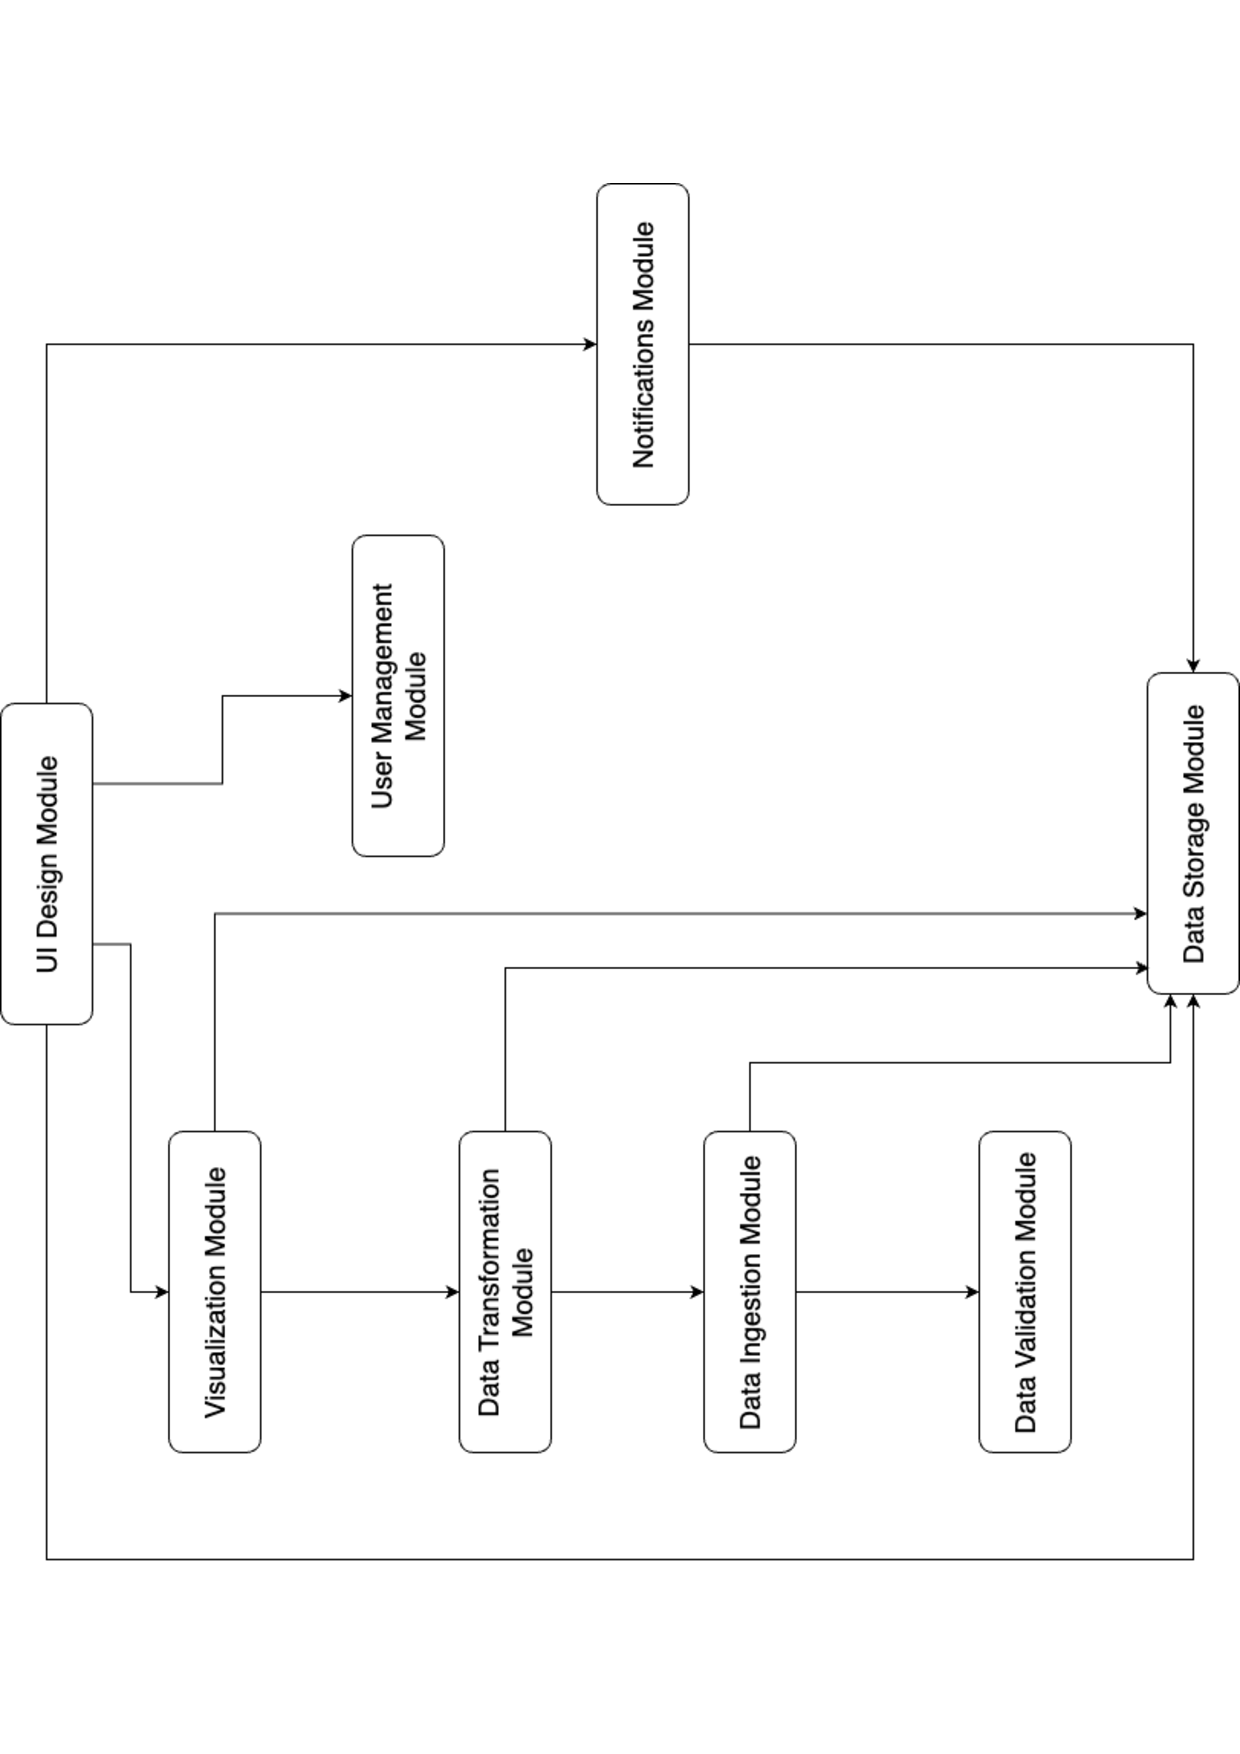
\includegraphics[angle=-90,scale=0.6]{Diagrams/uses hierarchy.pdf}
\caption{Use hierarchy among modules}
\label{FigUH}
\end{figure}

The diagram shows the following:
\begin{enumerate}
  \item The UI Design Module (\mref{mUID}) is at the highest level and uses multiple modules, 
  namely, the Data Storage Module (\mref{mDS}), the Visualization Module (\mref{mVI}), the User 
  Management Module (\mref{mUM}) and the Notifications Modules (\mref{mNO}).
  \item The Visualization Module (\mref{mVI}) uses the Data Transformation Module (\mref{mDT})
  and the Data Storage Module (\mref{mDS}).
  \item The Data Ingestion Module (\mref{mDI}) uses the Data Validation Module (\mref{mDV}) and 
  the Data Storage Module (\mref{mDS}).
  \item The Data Transformation Module (\mref{mDT}) uses the Data Ingestion Module (\mref{mDI})
  and the Data Storage Module (\mref{mDS}).
  \item The Notifications Module (\mref{mNO}) uses the Data Storage Module (\mref{mDS}).
  \item The Data Storage Module (\mref{mDS}) appears at the lowest level as it is used by many 
  other modules but does not depend on any other modules itself.
\end{enumerate}

\section{User Interfaces}
The following figures encompass key design mock-ups of the application
interface, created using Figma. These mock-ups are merely wireframes and do not
represent the final interface design of the application.
\begin{figure}[htbp]
  \centering
  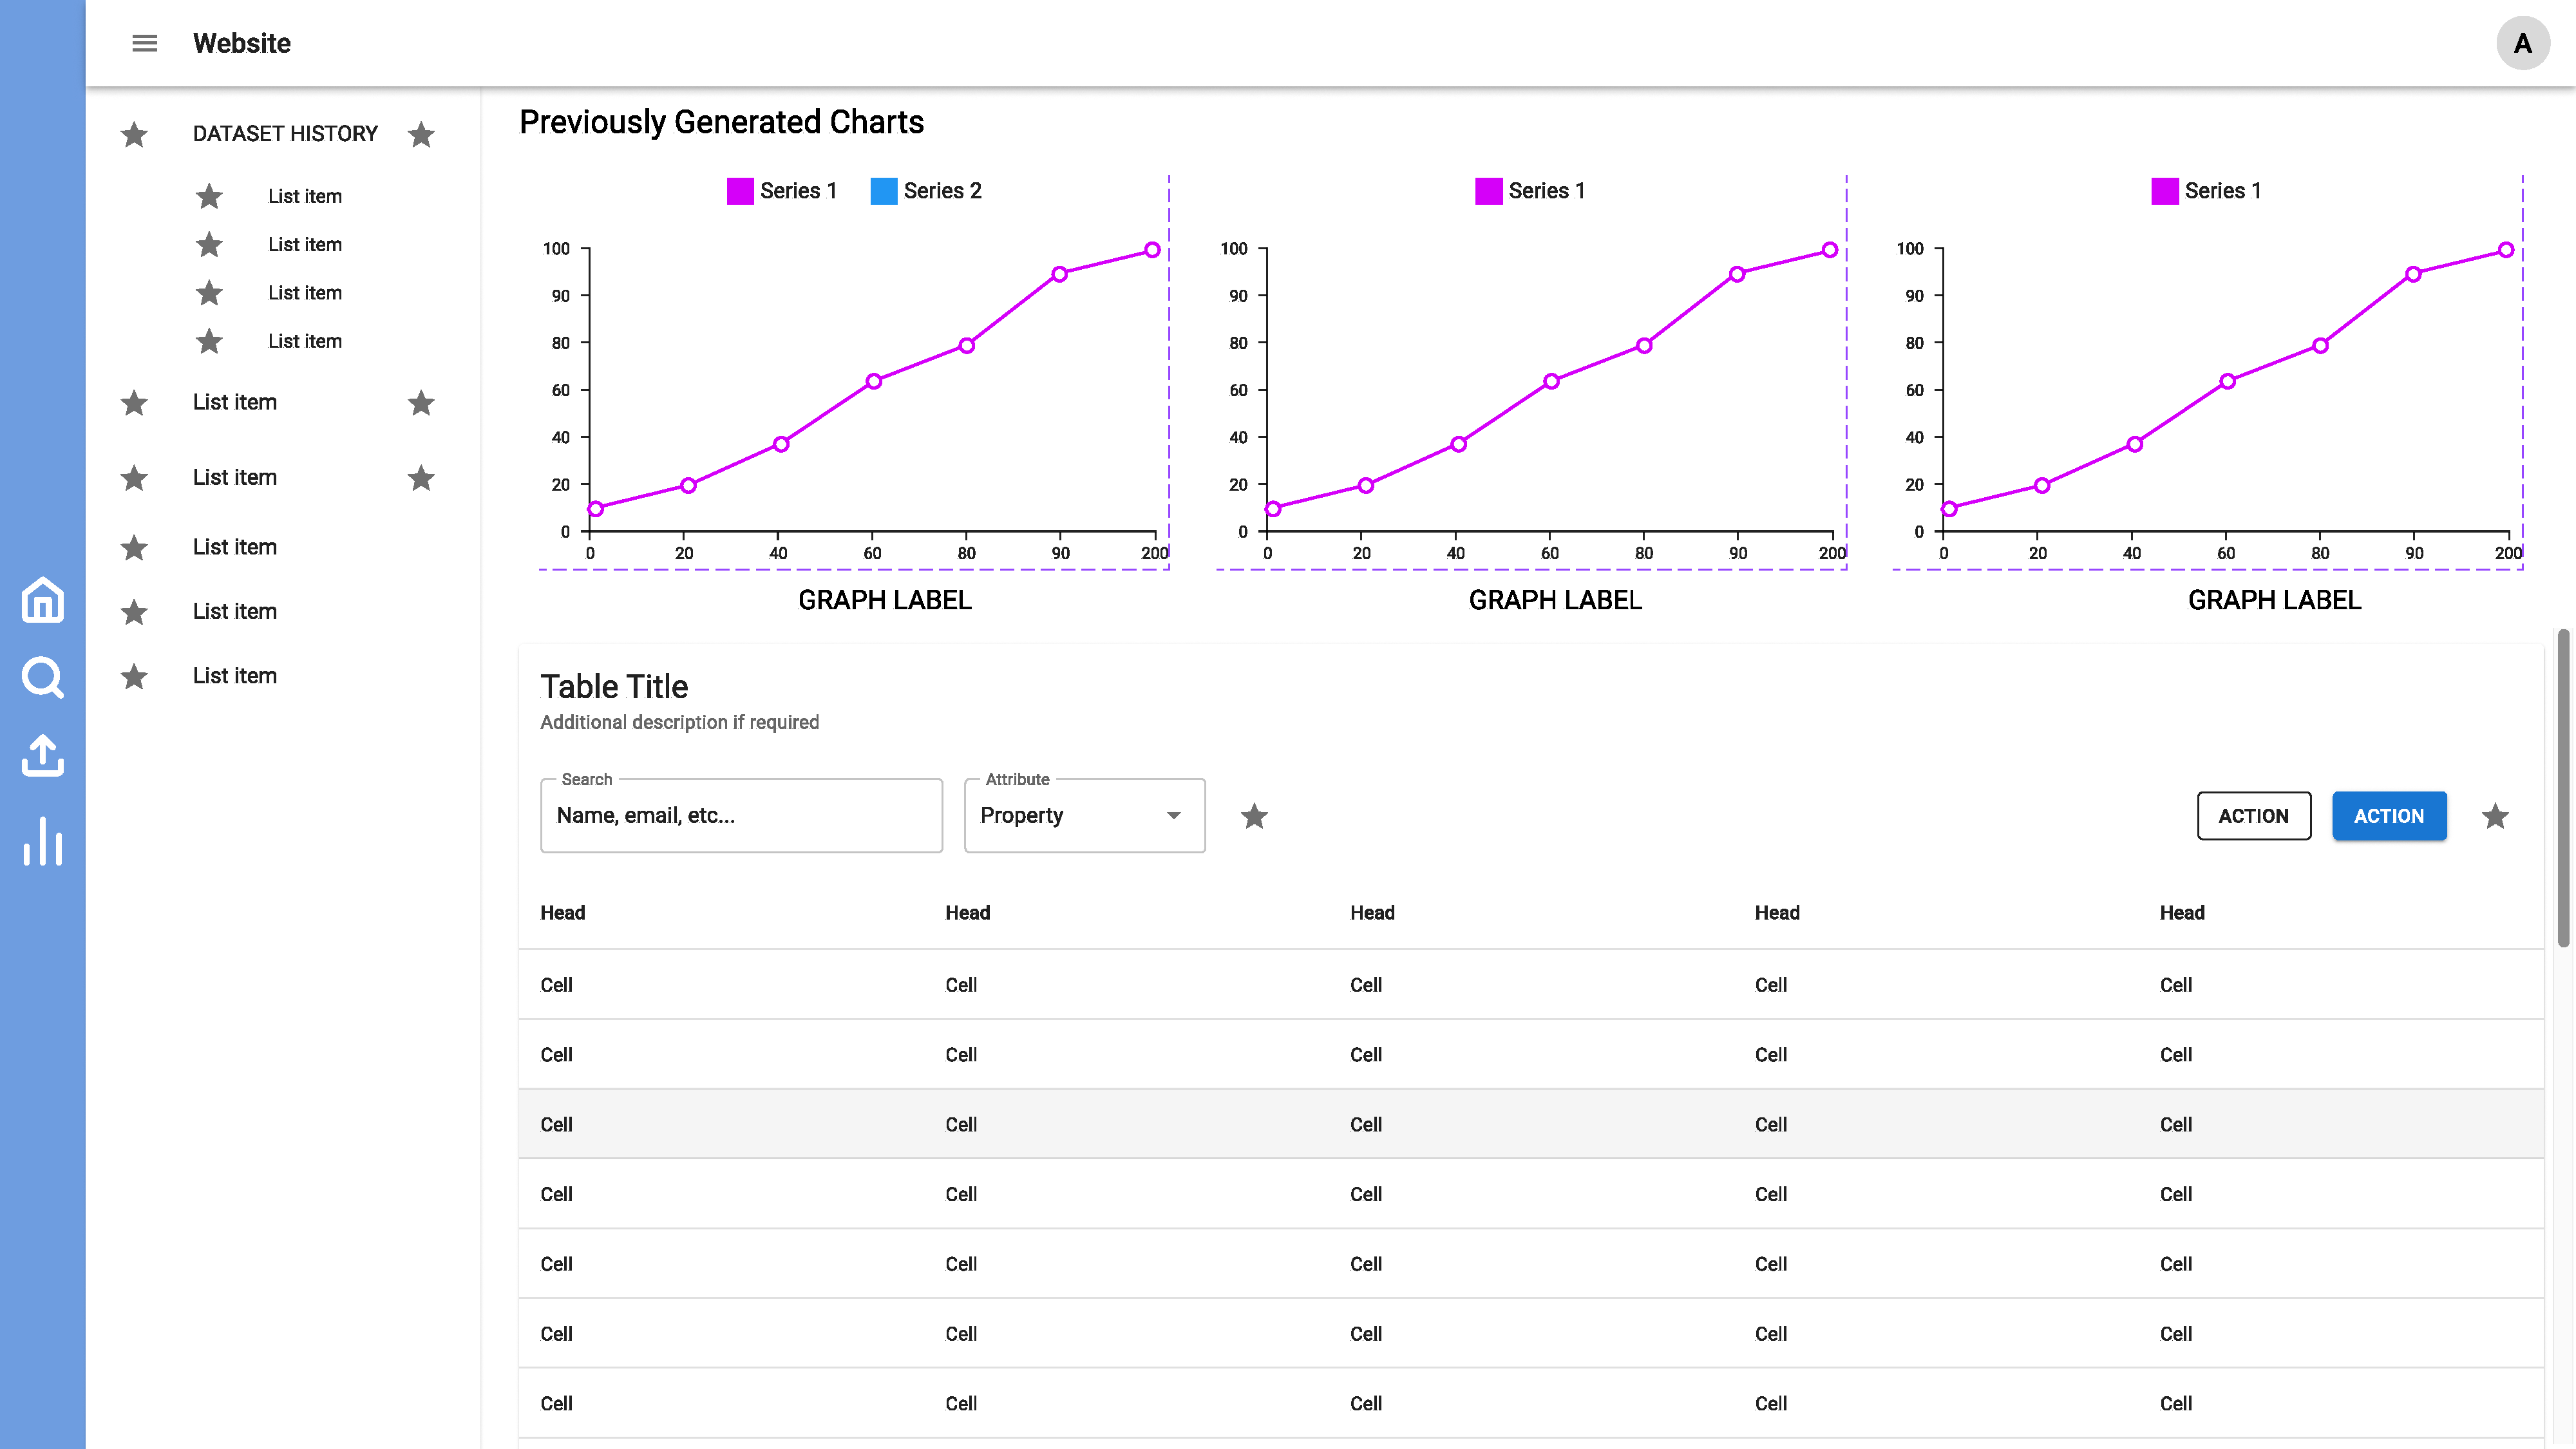
\includegraphics[width=\textwidth]{Figma/dashboard.pdf}
  \caption{The dashboard, or main home page of the application upon successful login.}
  \label{fig:FigUIDB}
\end{figure}

\begin{figure}[htbp]
  \centering
  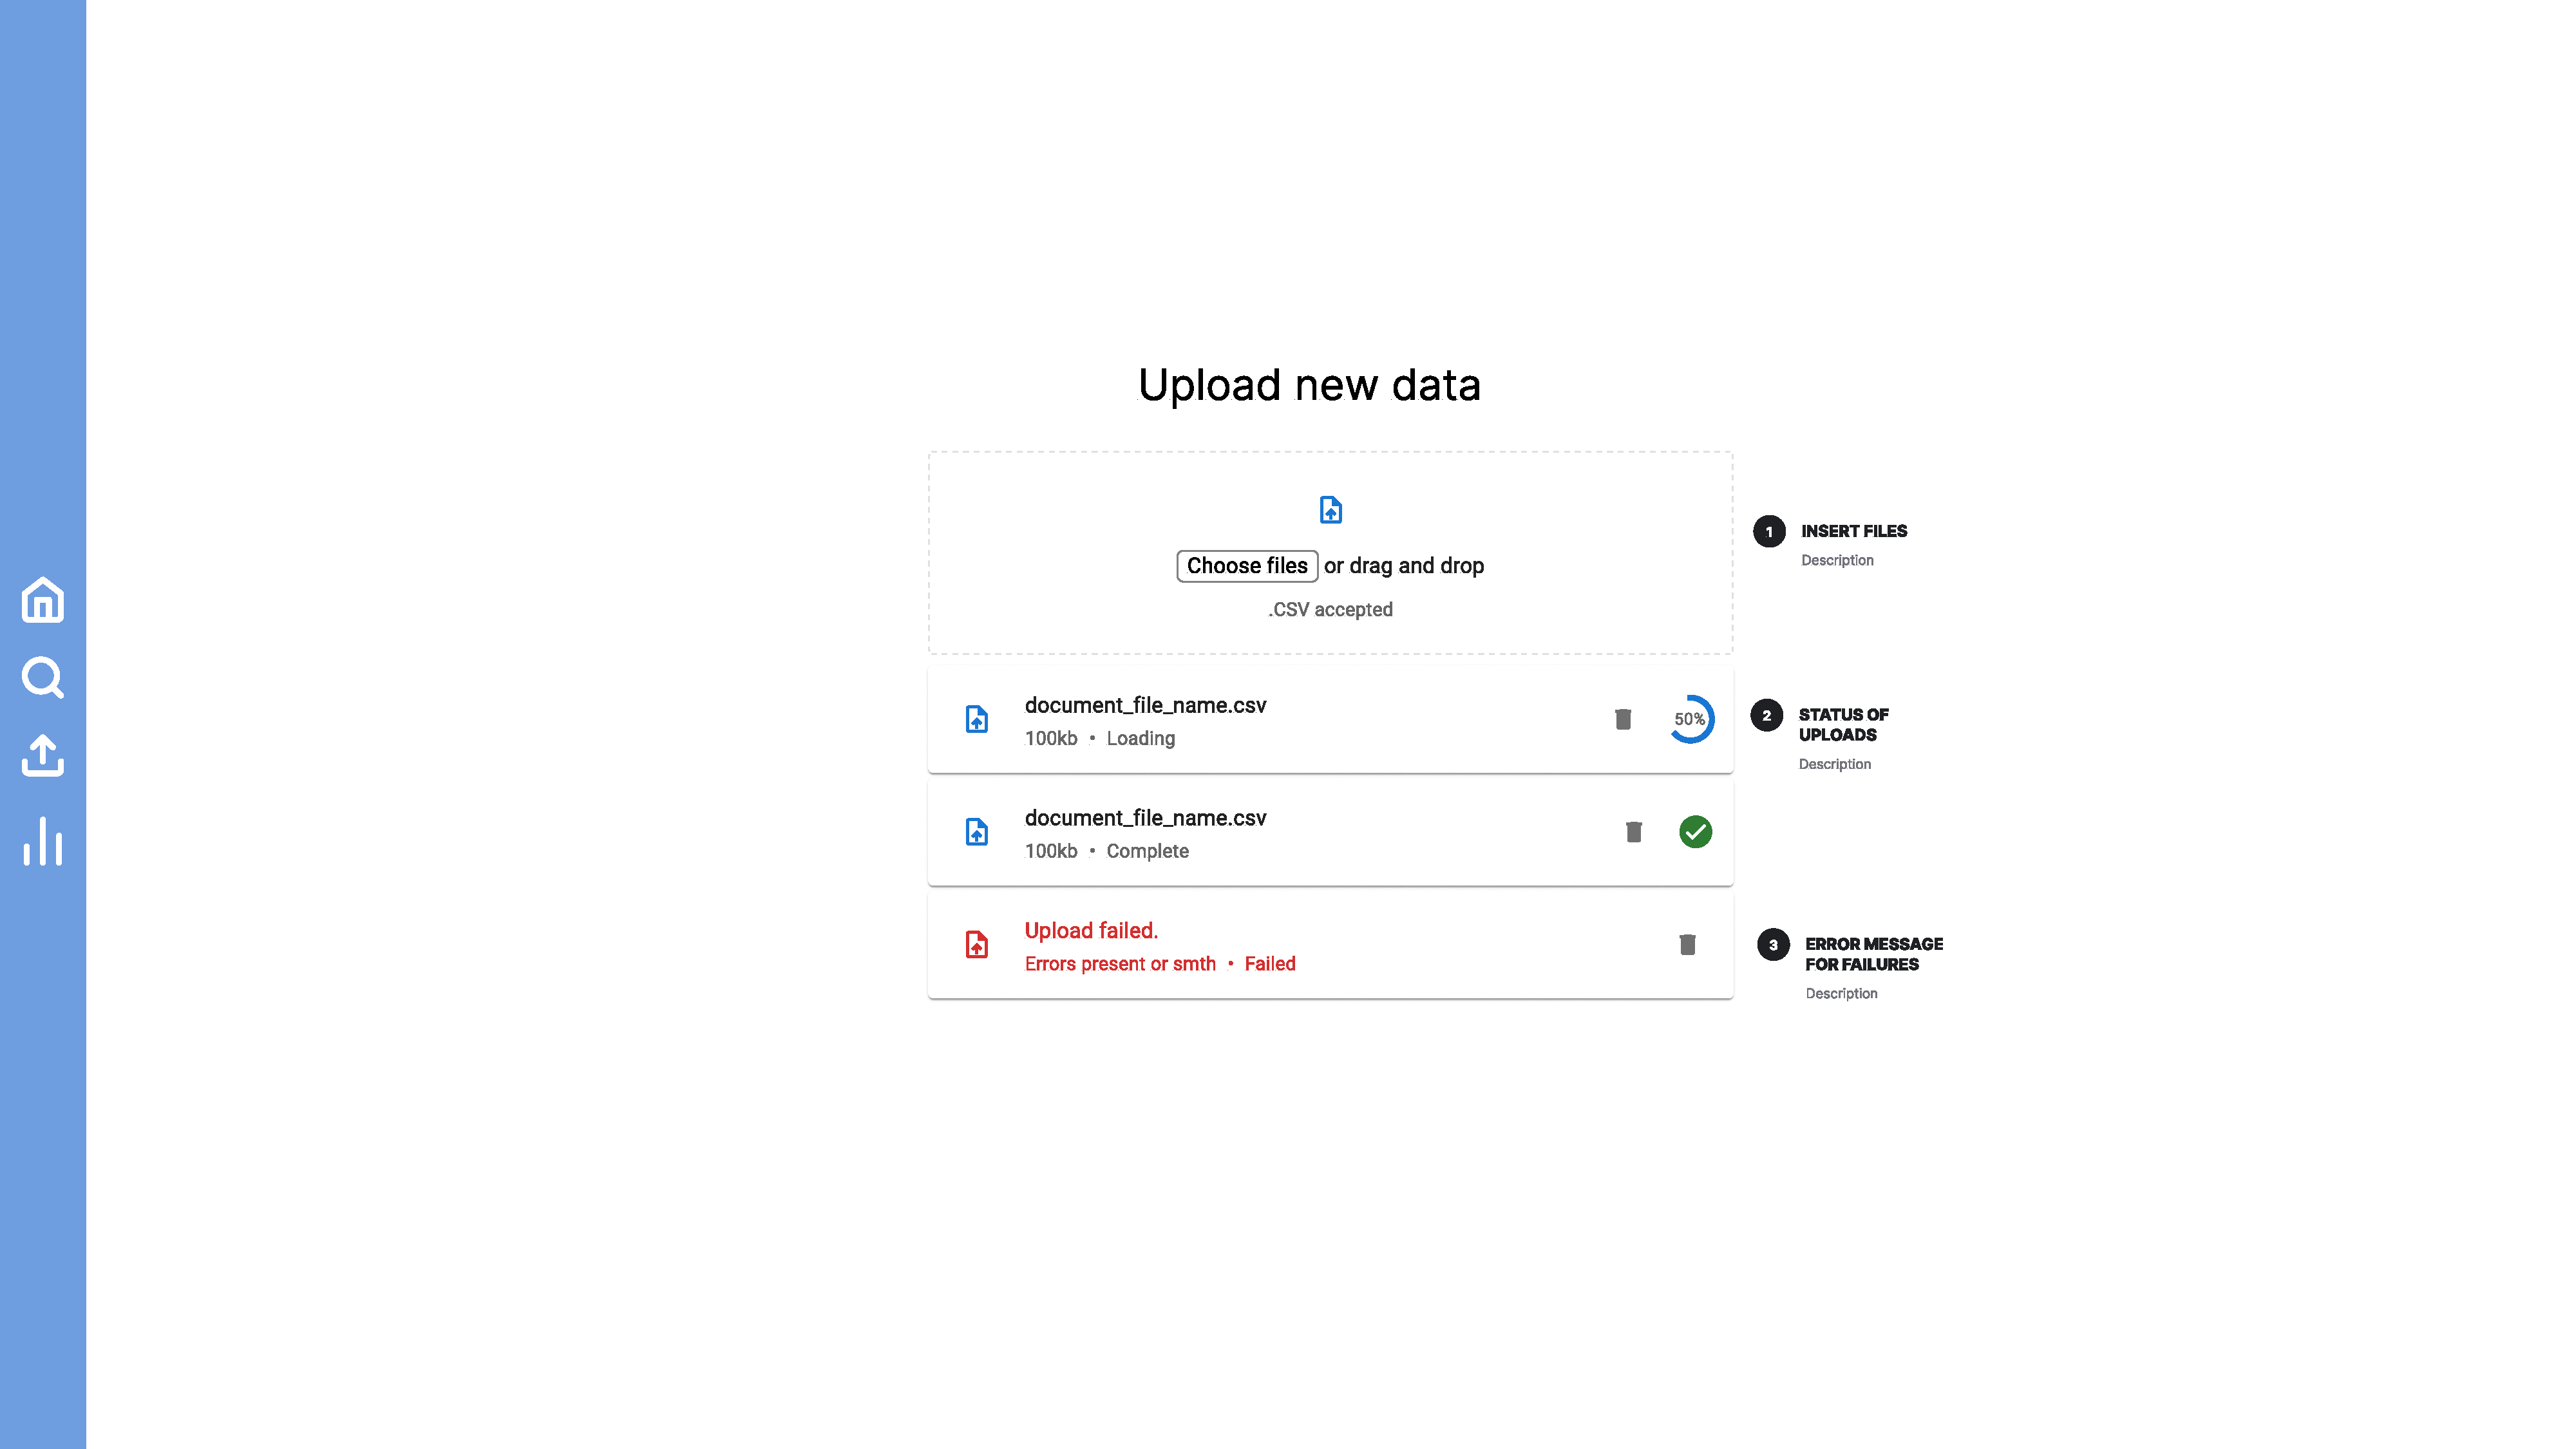
\includegraphics[width=\textwidth]{Figma/upload.pdf}
  \caption{The upload page for users to upload new experiment data files.}
  \label{fig:FigUIUP}
\end{figure}

\begin{figure}[htbp]
  \centering
  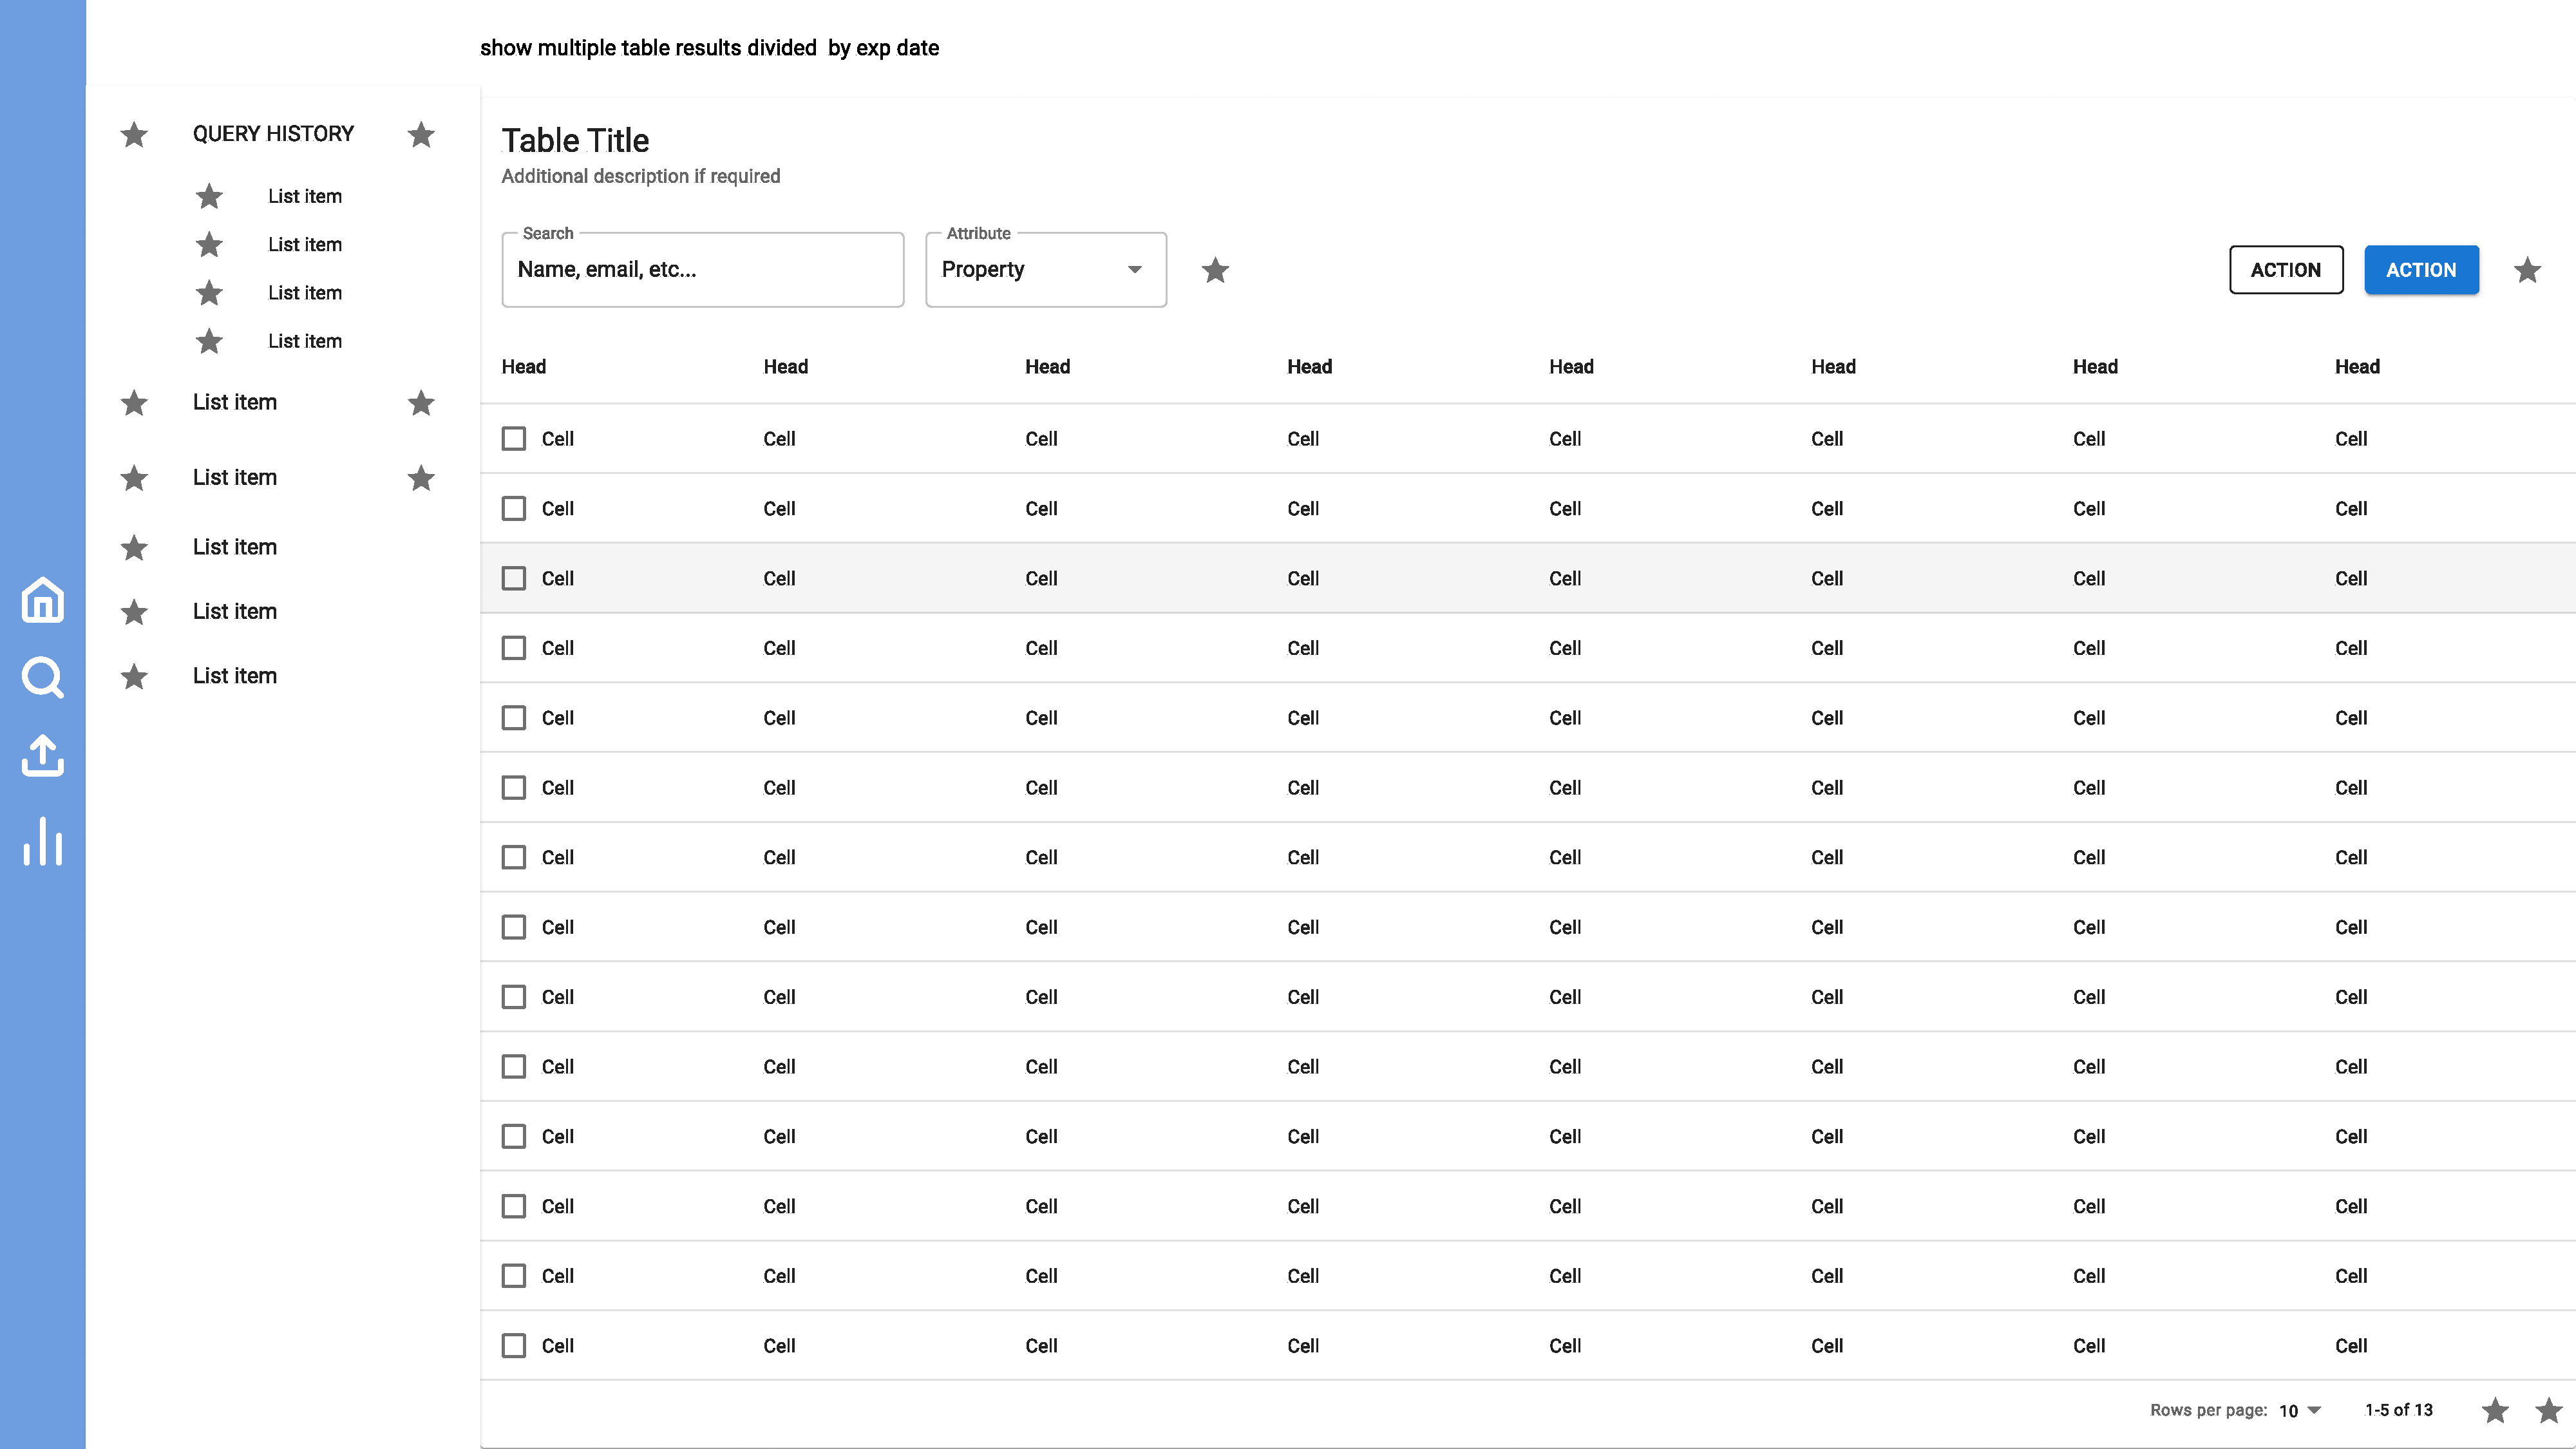
\includegraphics[width=\textwidth]{Figma/table.pdf}
  \caption{The main view page for querying and modifying data.}
  \label{fig:FigUITB}
\end{figure}

\begin{figure}[htbp]
  \centering
  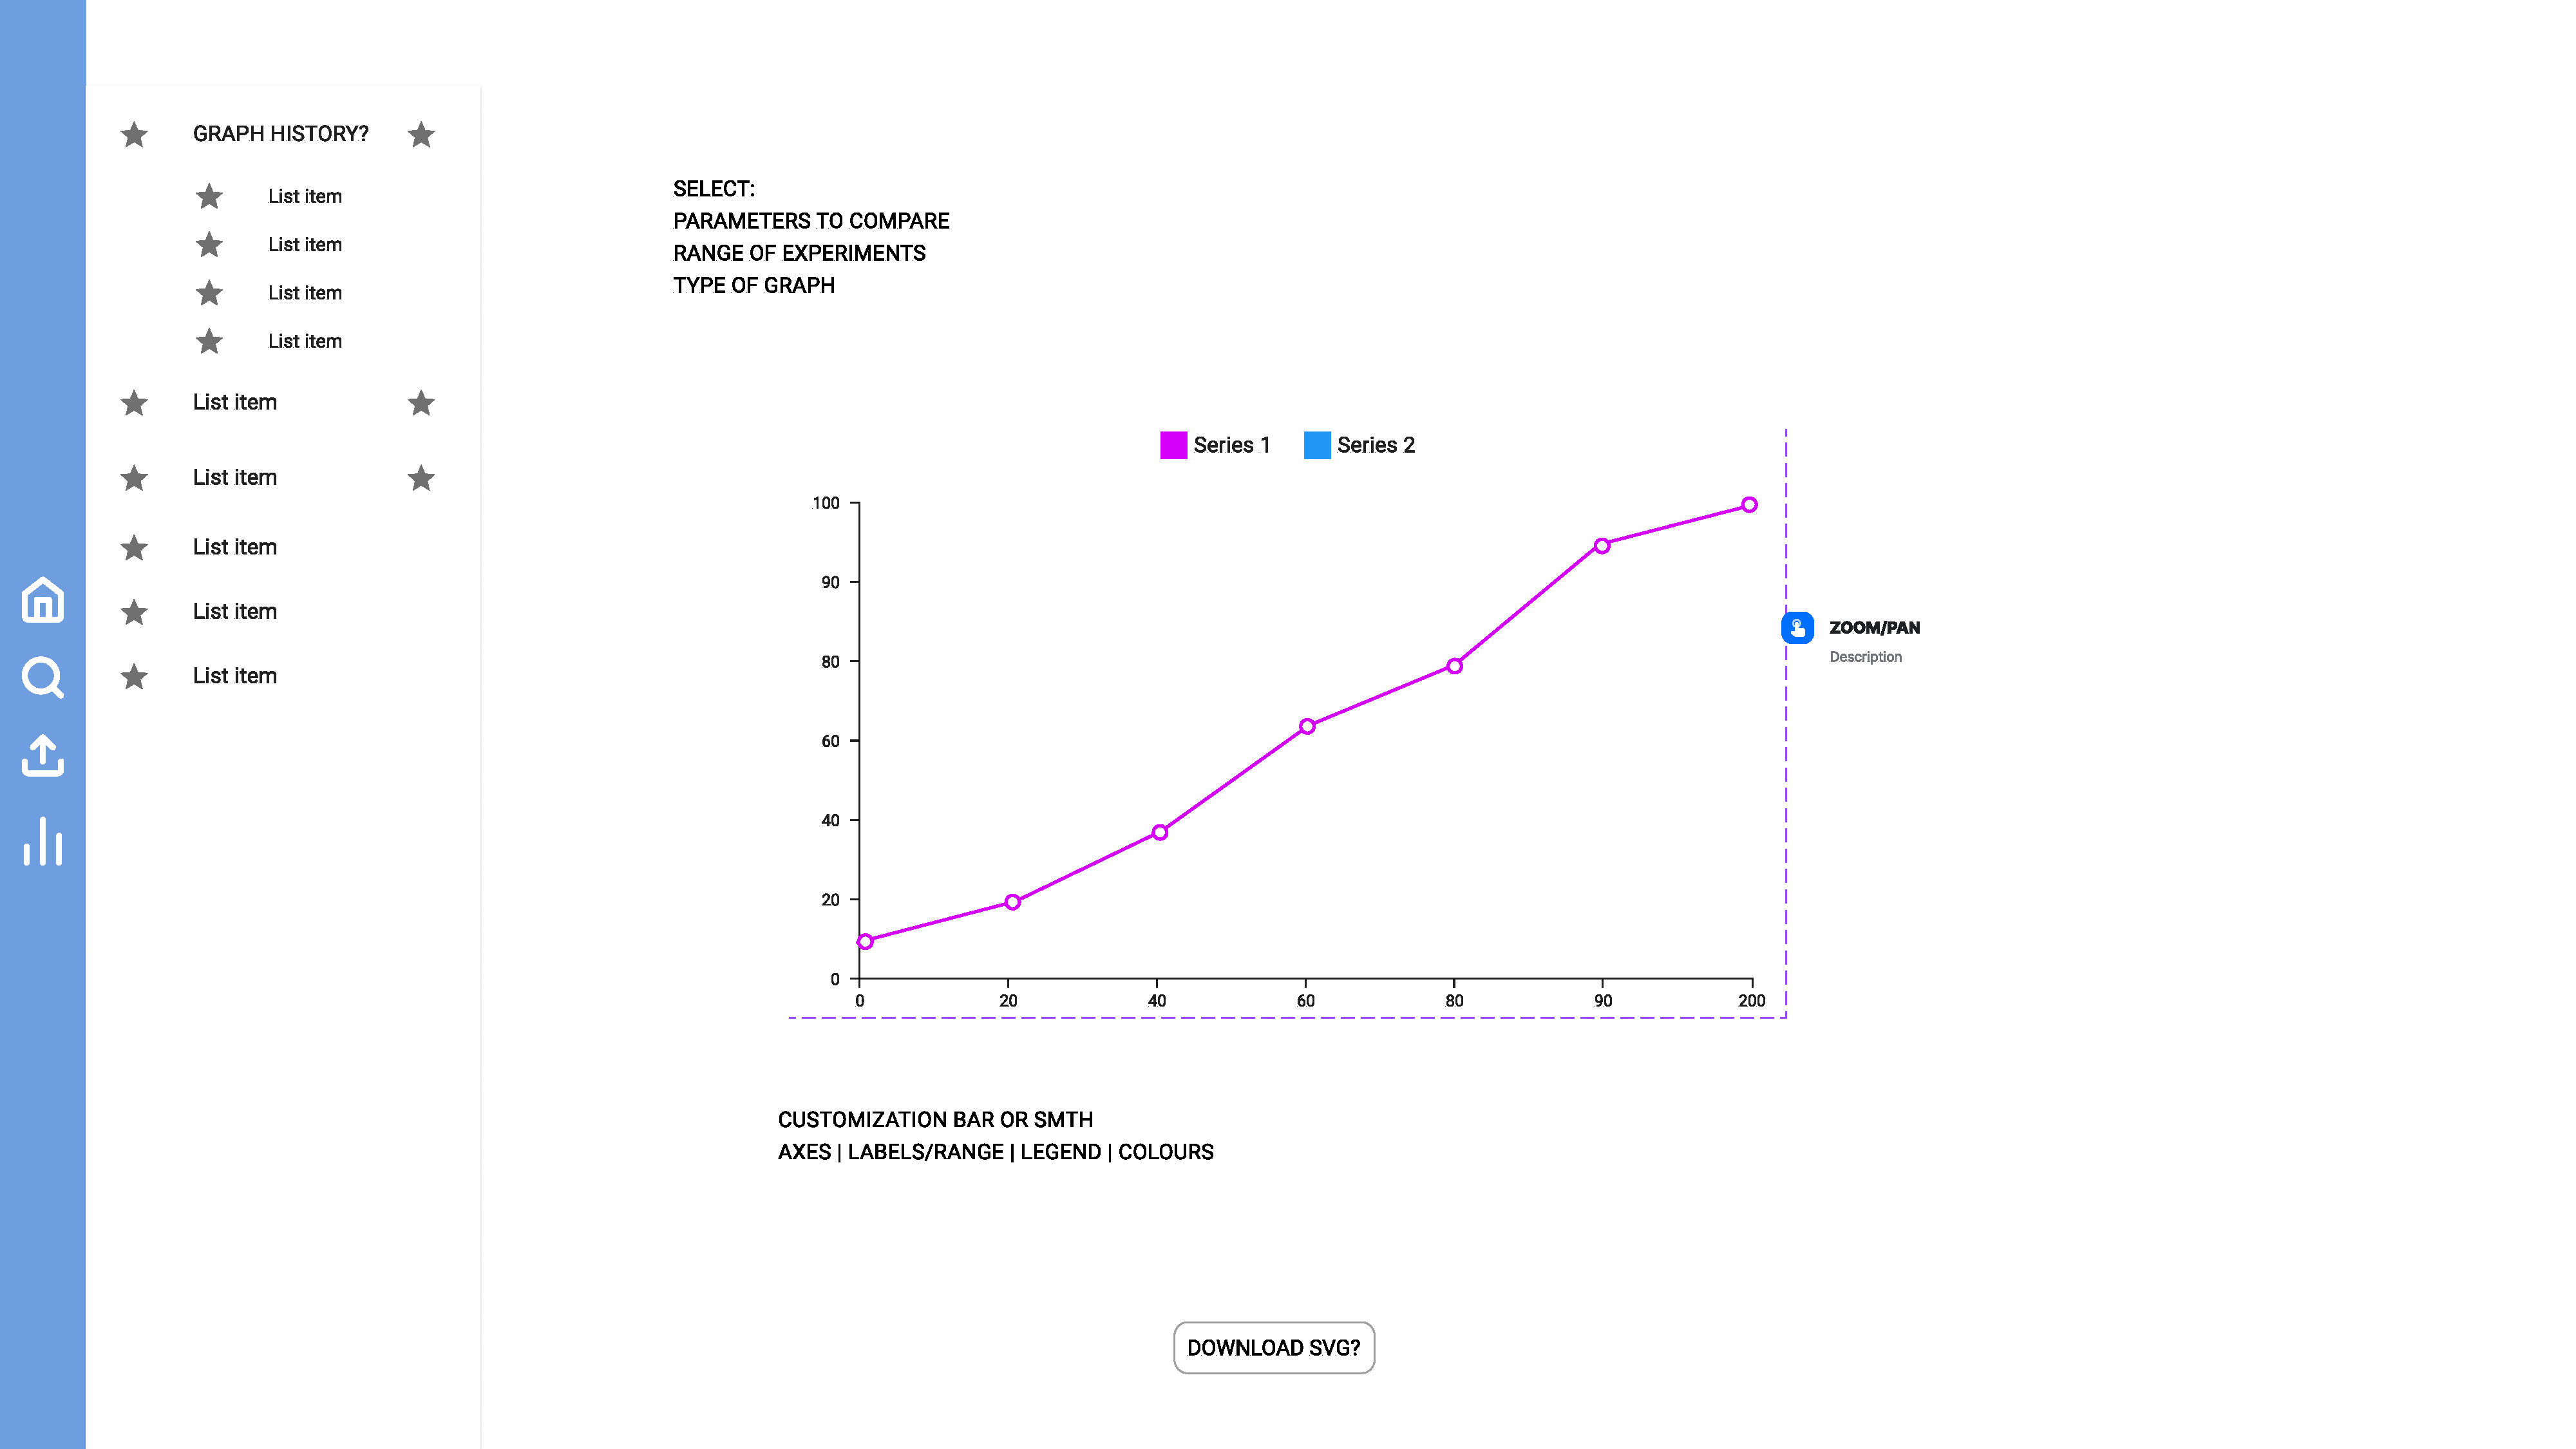
\includegraphics[width=\textwidth]{Figma/graphs.pdf}
  \caption{The main view page for generating and viewing visualizations of queried data.}
  \label{fig:FigUIG}
\end{figure}

\section{Timeline}
The following timeline details the implementation plan for Rev 0, outlining tasks down to 
the module level. Roles and responsibilities are clearly defined for each task, along with 
tentative time estimates. 
\subsection{Phase 1: Initial Setup and Core Architecture}
  \begin{table}[H]
    \centering
    \begin{tabular}{p{0.45\textwidth} p{0.13\textwidth} p{0.13\textwidth} p{0.17\textwidth}}
    \toprule
    \textbf{Task} & \textbf{Module(s)} & \textbf{Status} & \textbf{Responsible}\\
    \midrule
    Setting up a skeletal database. & \mref{mDS} & Done & Kate\\
    Creating algorithm to convert CSV files to JSON. & \mref{mDI} & Done & Jason\\
    Migrating all data to the database. & \mref{mDI}, \mref{mDS} & Done & Jason\\
    Testing the database and algorithm. & - & Done & Jennifer, Sumanya\\
    \midrule
    Setting up a CI/CD Infrastructure. & - & Done & Kate, Sumanya\\
    \bottomrule
    \end{tabular}
    \caption{Phase 1 Timeline}
    \label{TblT1}
    \end{table}

\subsection{Phase 2: Front End and User Roles}
  \begin{table}[H]
      \centering
      \begin{tabular}{p{0.45\textwidth} p{0.13\textwidth} p{0.17\textwidth} p{0.17\textwidth}}
      \toprule
      \textbf{Task} & \textbf{Module(s)} & \textbf{Status} & \textbf{Responsible}\\
      \midrule
      Drawing wireframes and finalizing design elements. & \mref{mUID} & Done & All\\
      \midrule
      Making a login page. & \mref{mUID}, \mref{mUM} & Weeks 14-16  & Kate\\
      Creating the upload screen. & \mref{mUID}, \mref{mDI} & Weeks 14-16 & Jason\\
      Building key frontend components including navigation and basic layouts. & \mref{mUID} &
      Weeks 14-16 & Jennifer\\
      \midrule
      Develop user login, registration and session management. & \mref{mUM} & Weeks 15-17 & Kate\\
      \bottomrule
      \end{tabular}
      \caption{Phase 2 Timeline}
      \label{TblT2}
    \end{table}

\subsection{Phase 3: Data Ingestion Pipeline and Core Analytics Engine} 
    \begin{table}[H]
      \centering
      \begin{tabular}{p{0.45\textwidth} p{0.13\textwidth} p{0.17\textwidth} p{0.17\textwidth}}
      \toprule
      \textbf{Task} & \textbf{Module(s)} & \textbf{Status} & \textbf{Responsible}\\
      \midrule
      Implementing the pipeline to handle data import, transformation and storage. & 
      \mref{mDI}, \mref{mDT}, \mref{mDS} & Weeks 16-17 & Jason, Sumanya\\
      \midrule
      Migrate basic analytical functionalities. & \mref{mDT} & Weeks 15-17  & Sumanya\\
      Basic testing to ensure data integrity.  & \mref{mDV} & Week 15 & Jennifer\\
      Implementing data validation rules. & \mref{mDV}, \mref{mDT} & Weeks 15-17 & Kate\\
      \bottomrule
      \end{tabular}
      \caption{Phase 3 Timeline}
      \label{TblT3}
    \end{table}

\subsection{Phase 4: Setting-up Dashboards and Connecting Components}
    \begin{table}[H]
      \centering
      \begin{tabular}{p{0.45\textwidth} p{0.13\textwidth} p{0.17\textwidth} p{0.17\textwidth}}
      \toprule
      \textbf{Task} & \textbf{Module(s)} & \textbf{Status} & \textbf{Responsible}\\
      \midrule
      Use processed and transformed data to generate graphs. & \mref{mDT}, \mref{mVI} & Week 18 & Jennifer, Kate\\
      \midrule
      Connect frontend, backend and data modules via APIs. & - & Week 18  & Jason\\
      Integration testing to ensure smooth system operation. & - & Week 18 & Sumanya\\
      \bottomrule
      \end{tabular}
      \caption{Phase 4 Timeline}
      \label{TblT4}
    \end{table}

\bibliographystyle {plainnat}
\bibliography{../../../refs/References}

\newpage{}

\section*{Appendix --- Reflection}
The information in this section will be used to evaluate the team members on the
graduate attribute of Problem Analysis and Design.

\begin{enumerate}
  \item \textbf{What went well while writing this deliverable?}\\
  \newline
  While writing this deliverable, the clear structure and organization of the module guide 
  worked well allowing us to track and understand the project's timeline. Having to brainstorm 
  all likely and unlikely changes that could have major impacts on the implementation timeline 
  of the project, made us more cognizant about the need for flexibility and adaptability when 
  we code. The code, in addition to being modular, must also be scalable.
  \item \textbf{What pain points did you experience during this deliverable, and how
    did you resolve them?}\\
  \newline
  Through the course of our previous software engineering courses, we had formed the habit of 
  figuring out the structure and needed variables, constants, etc. for each module as we begin 
  coding the module if this information wasn't already included in the MIS. We realize that writing 
  an MIS as you go defeats the purpose of documentation but for smaller projects, it is often easier 
  that way.\\
  \newline
  Given that, coming up with intricate implementation details for each module, down to what each 
  routine would be named or what environment variables must be considered was tricky at first since 
  we had not start the implementation of these modules yet. However, having these thoughtfully 
  articulated details for when we start implementing would make our jobs much easier. This would avoid 
  back and forth and ensure consistency amongst the team even if two or more team members are working on 
  different parts of a module at the same time.

  \item \textbf{Which of your design decisions stemmed from speaking to your client(s)
  or a proxy (e.g. your peers, stakeholders, potential users)? For those that
  were not, why, and where did they come from?}\\
  \newline
  Most of the frontend-related decisions stemmed from our conversations with our clients. Our team 
  carefully put together a vision board of sorts to get an idea of what kind of layout the client would 
  prefer. After getting some initial feedback on their preferred designs, we drew up wireframes in 
  Figma to ensure that there is consistency amongst the various pages being implemented by different 
  team members.\\
  \newline
  For other back-end related components, most of our decisions were either made internally by the team or 
  based off our conversations with our TA during the Proof of Concept feedback session and other informal 
  presentations. We made these decisions based off of our learnings from courses like SFWRENG 2AA4, 3RA3 and more.

  \item \textbf{While creating the design doc, what parts of your other documents (e.g.
  requirements, hazard analysis, etc), if any, needed to be changed, and why?}\\
  \newline
  Although the SRS helped immensely while writing the design document, no parts of it or other 
  documents had to be changed. However, after receiving feedback on the scope of our AC and UC, our team will 
  likely have to revisit the \href{https://github.com/SumanyaG/Alkalytics/blob/main/docs/HazardAnalysis/HazardAnalysis.pdf}{Hazard Analysis}
  and re-evaluate the risks, including some of the newly brainstormed UCs.

  \item \textbf{What are the limitations of your solution?  Put another way, given
  unlimited resources, what could you do to make the project better? (LO\_ProbSolutions)}\\
  \newline
  Given unlimited resources—particularly additional time, personnel, and development support—our team would address several current 
  limitations in the Alkalytics system, especially those related to modularity, completeness, and maintainability.\\
  \newline
  Currently, several critical components—represented as orange leaf modules in \ref{fig:FigMH}—are not implemented in Revision 0 due 
  to strict timeline constraints. These include modules responsible for advanced data visualization, automatic calibration routines, 
  and persistent cloud-based data storage. Their absence limits the overall functionality, real-time responsiveness, and scalability of 
  the system.\\
  \newline
  From a software engineering standpoint, the current implementation exhibits tight coupling between certain components, particularly 
  between data parsing, validation, and processing. This violates the principle of separation of concerns and makes future updates or 
  substitutions (e.g., using a different input format) more difficult. With more resources, we would refactor these modules to follow 
  stricter encapsulation—ensuring each component has a well-defined interface and hides its internal logic.\\
  \newline
  Additionally, validation logic is currently focused on domain-specific checks and lacks a fully generic, extensible validation framework.
  A more modular design could support pluggable validation rules, improving reusability across different datasets or future input types. 
  We would also strengthen information hiding practices by isolating error handling and logging mechanisms from the core logic, making the 
  system easier to test and debug.\\
  \newline
  Finally, our stretch goals from the Problem Statement and Goals document—such as automated alert systems, remote monitoring integration, 
  and user customization support—would be implemented. These features require additional layers of abstraction and service integration that 
  would benefit greatly from a well-modularized and extensible codebase.\\
  \newline
  In summary, with additional resources, we would improve the system's modularity, promote cleaner separation of concerns, enhance 
  extensibility, and better align with industry-standard software engineering practices.\\

  \item \textbf{Give a brief overview of other design solutions you considered.  What
  are the benefits and tradeoffs of those other designs compared with the chosen
  design?  From all the potential options, why did you select the documented design?
  (LO\_Explores)}\\
  \newline
  In considering other design solutions, we evaluated approaches such as a monolithic architecture 
  versus a modular design, as well as centralized versus distributed data management system. One 
  alternative was a monolithic structure where all components were tightly integrated, which could simplify the 
  initial setup but would become difficult to scale and maintain as the project grew. Another option was a fully 
  centralized database, which could offer easier data management initially but could also introduce a single 
  point of failure and scalability concerns.\\
  \newline
  After weighing the benefits and trade-offs, the modular design with distributed tasks and responsibilities 
  was chosen. This approach allows for better scalability, easier maintenance, and flexibility in task management.
  The modular setup also ensures that changes or improvements to one part of the system don't disrupt the entire project.
  Additionally, it helps in assigning clear roles and responsibilities in the design which in turn, helps with accountability
  and project management.\\
  \newline
  The decision to select this documented design was driven by its adaptability and long-term sustainability. It allowed for 
  easier integration of new modules and improvements, aligned well with our team's collaborative workflow, and mitigated the
  risk of potential bottlenecks or system failures. Therefore, the modular design was deemed the best fit for the project's needs,
  offering both flexibility and stability.
\end{enumerate}

\end{document}